%!TeX program=pdflatex
%!TeX encoding=utf8
%!TeX spellcheck = en_US
%!TeX root = ../../messageVortex.tex
\partepigraph{Atoms are very special: they like certain particular partners, certain particular directions, and so on. It is the job of physics to analyze why each one wants what it wants.}{Richard P. Feynman}
\part{Analysis of \MessageVortex}\label{sec:analysis}
In \cref{sec:adversary}, we described two different kinds of adversaries. These adversaries require different properties to be fulfilled. 

An observing adversary is the less restricting one. While this adversary observes all traffic, he does not disrupt communication. Instead, he uses all available information to collect data about all items of interest (\defref{IoI}). He may do this, for example, by collecting inside or outside information about all message flows he may encounter. He may use this information and assign it to specific individuals or groups of individuals.

A censoring attacker is far more dangerous to our system as he does not only observe the system, but he may systematically suppress freedom of speech and all related technology. As he has the means and the technical know-how, he may try, apart from observing, to discover systems communicating illegally either by observation or by infiltration of systems. He may furthermore track down individuals within reach and prosecute them. All other illegal system participants may be either identified and blacklisted or even attacked either by infiltrating their systems or by effectively launching DoS attacks against those systems.

In the following sections we will analyze aspects of confidentiality, integrity, and availability for our system and highlight differences in terms of the different adversaries.

\chapter[Identification of Attacks and Mitigations]{Identification of Possible Attack Schemes and Mitigation}\label{sec:attacks}
In this chapter, we take the attacks identified in \cref{sec:wellKnownAttacks} and analyze our protocol on whether it is susceptible to such attacks or not.

\section{Static Attacks}
Static attacks typically address weaknesses within a protocol design. The following attacks are typically used to attack protocols similar to our proposal.

A \VortexMessage{} itself is crafted in such a way that for a routing node, only minimal effort is sufficient to obtain a short-lived pseudonym (\defref{eID}) of the sending party of a transmission. The Operations $ K_{msgN}=D^{K^{1}_{host}}\left(P\right)$ and $HEADER=D^{K_{msgN}}\left(H\right)$ are sufficient to identify message senders. Unknown senders may be discarded without further processing. Known senders may be identified as legitimate and processed further. Known misbehaving identities and message duplicates may be discarded. In section{sec:analysisBlendingAndTransport}, we will emphasize on approaches allowing identification and censorship of \VortexMessages{} and \VortexNodes.

Bugging and tagging attacks are similar in terms that both try to follow a message to its final recipient. While the goal is similar, the approaches are entirely different.

We refer to a bugging attack as an attack, which discloses the recipient by forcing him to do a disclosing action. Such an action may be the lookup of an unusual DNS record, verification of some identifiable data (e.g., an OCSP request to verify a certificate), or downloading an external image induced by an attacker.

A tagging attack allows an adversary to follow an attribute of a message through a network and, thus, uncover members of a network, subsequent messages, or even a final recipient.

Static information leaking of the protocol is another possibility of how an adversary may learn \defref{IoI}s on a network. Routing nodes are a vital part of any anonymity network. The most comfortable assumption is to trust nodes. In our case, we explicitly distrust routing nodes. This means that we must identify and judge upon the footprint of available information to such routing nodes, which is done in \cref{sec:staticAnalysis}. Especially in an environment of a censoring adversary, the undetectability of a \VortexNode{} is crucial, as any detectability may lead to a shutdown or even repression. We will look in \cref{sec:analysisBlendingAndTransport} how to identify involved messages and nodes.

\section{Dynamic Attacks}
Dynamic attacks usually involve an active adversary injecting malicious traffic. They are quite often paired with statistical approaches to discover properties of the system otherwise not available to an observer. 

An active adversary may attack the transport layer. Most of the transport layers are not able to react to message flooding. Therefore, it is easy to attack a transport layer with a flooding attack, such as a distributed denial of service (DDoS) attack. Due to the nature of the protocol, we cannot create additional protection on the transport layer as such modification would require a modification of the transport layer. We will analyze in \cref{sec:dynamicAnalysis} the impact on the \MessageVortex{} system.

We have identified the following attacks relevant to our system:
\begin{itemize}
	\item DoS attacks against the transport system
	\item DoS by traffic replay
	\item DoS by traffic generation
	\item Attacking a single ephemeral identity of a \VortexNode
	\item Denial of service by exhausting quotas or limits
	\item Attacking sending and receiving identities of the \MessageVortex{} system
	\item Traffic highlighting or traffic analysis
	\item Recovery of previously carried out operations
\end{itemize}

An active adversary may not follow the protocol and modify any parts of the message. The following paragraphs reflect different kinds of behavior and how they affect the messages and the system as a whole.

An adversary may not follow the blending specification. If he uses a less secure specification, an independent third party observer may follow traffic. Such a behavior is not sensible as such a node may directly send all the knowledge to such a collaborating node. If a  target node does not support the chosen blending method, the partial message path becomes interrupted. A possible redundancy in the path may recover the message from such a case.

Traffic replay is a common way to highlight traffic in many systems by replaying the same traffic and increasing the signal to the noise ratio of a system. In our case, we can use the replay of a \VortexMessage block to increase the traffic to a node. After decoding the header, a \VortexNode{} identifies the block as a repeated block and rejects further processing. 

An adversary may replay blocks with varying content. Such replays will not result in a DoS attack as the quota is not decreased on replayed messages (see \cref{fig:msgReceiveProcessing}).

An adversary may first collect identities and quotas and use them later in a coordinated attack to force the node processing. The adversary may increase the impact by using large payloads and processing them in a costly manner. A possibility is to make extensive use of $addRedundancy$ or encryption operations. Furthermore, an attacker may attack the memory by distributing the message throughout the workspace to exhaust the routers' runtime memory.

As a router is free to process the operations of identity, he may discard an ephemeral identity and all associated resources at any time. Misbehaving or suspected misbehaving nodes may, therefore, be stopped. On the other hand, we are unable to prevent an adversary from allocating new identities. We may, however, work with multiple local host keys and distribute them according to the trust. A known party or someone trusted by them might receive a key different from a publicly advertised key. This identity key may be dropped at any time and distributed to further parties again with an identity update. We may even subdivide trusted parties into several groups by updating them with different new host keys to identify misbehaving routers without knowing them. 

\chapter{Static Analysis}\label{sec:staticAnalysis}
\section{Analysis of the Blending and Transport Layer}\label{sec:analysisBlendingAndTransport}
The blending layer is one of the key factors for confidentiality in an environment affected by a censoring adversary. We refer to the confidentiality of the presence of a \VortexNode{} as detectability. Detectability of messages and systems, in consequence, leads to the ability of censorship by an adversary. We assume that general censorship on the transport layer (e.g., by blocking all SMTP traffic) is not an option.

In an observing adversary environment, confidentiality regarding the presence of messages is not required, as we defined in those environments legal to use \MessageVortex. In such environments, plain embedding may be used at any time.

\subsection{Identifying a \VortexMessage{} Endpoint}
Depending on the blending method, a single, identifiable message is sufficient to identify a \VortexNode. Detectability depends on various factors, such as:

\begin{itemize}
	\item Broken internal file structure (due to plain blending)
	\item Uncommon high entropy in a structureless file
	\item Unrelated message flow (see~\cite{oakland2013-parrot})
	\item Non-human behavior on the transport layer (e.g., message traffic 24x7)
\end{itemize}

If an endpoint is successfully identified, then all peering endpoints of the same protocol may be identified as well by following the message flow. However, this does not enable an adversary to inject messages as the host key is not leaked. 

Assuming a global observer as an adversary and unencrypted traffic, %FIXME2 is the global observer both? No...?
 he might discover the originating routing layer and thus identify it as \VortexNode{} by following traces of the transport layer. However, in most protocols this address is spoofable and not a reliable source for the originating account.

As we specified machine communication for our messages, the Dead Parrot problem~\cite{oaklan/d2013-parrot} is not an issue as it only follows human communication. Thus, our system does not have to pass a Turing test. Having messages sent with a non-human behavioral pattern (e.g., 24x7) is, therefore, not an issue either, as well as sending unrelated messages to an unstable set of endpoints. 

\subsection{Analysis of the F5-Embedding Method}
A routing node must embed the \VortexMessage{} into a generated image. Sending the same image multiple times without any generated content will look very suspicious as the same image sent multiple times but with a different fingerprint is not normal behavior. While we may adopt message sending code from open source products, it is not perfect as anyone may know what types of messages are affected. In return, this means that any message not heavily customized is suspicious. To make things worse, modifying the text may be relatively easy while modifying the content of generated imagery is much more difficult.

From the technical point of view, the specification for the blending layer is complete. By specifying only one steganography algorithm, we cannot switch algorithms, which makes the blending layer potentially weaker as there is no seconding algorithm such as PQt providing crypto-agility. While F5 has been available for many years, no paper has been published proving the algorithm's detectability. F5 was analyzed among others and showed remarkable resistance to conventional attacks. Detectability is depending on the density of embedded data. A payload of 5--10 percent is currently not deemed detectable in a real-world environment~\cite{fridrich2007statistically}. Many other algorithms such as nsF5, PQt/PQe, HUGO~\cite{pevny2010using}, S-UNIWARD~\cite{holub2014universal}, MiPOD~\cite{sedighi2015content}, or HILL~\cite{li2014new} have been evaluated but offering a solid implementation is nowadays rare. An implementation in Java was not available for any of the mentioned algorithms. Considering that it is far harder to provide a solid implementation than some emulation code for academic purposes, the lack of this is understandable yet makes it very difficult to either incorporate algorithms or test their robustness under realistic conditions.

Hiding a \VortexNode{} from a censoring adversary means that we have to generate credible traffic for sending messages containing imagery roughly 10--20 times as big as the embedded payload. The \defref{carrier message}s require properties, which makes them assignable to a service instead of a user as the source of the message (e.g., personalized evaluation documents, status information, password recovery messages, or statistics). These messages should have constantly sized attachments as it would be typical for a process to generate messages always following the same patterns. Such a size restriction for an embedding image is one of the caveats for larger messages as adaptive image size is easily detectable by an adversary. 

\section{Analysis of Plain Embedding}
It is undeniable why a file treated with plain embedding is easily identifiable as a broken or tampered file. Its use is undeniable when looking at the fact that almost 100\% of the carrier media may be used. While the information may remain parseable, its content is no longer sensible to a human and thus at least suspect. Therefore, plain embedding is not suitable for use in environments with a censoring adversary and may be seen as very weak obfuscation in an observing adversary's environments.

We wanted to know if there is a simple method to detect the modifications of such a file. While most of the analysis method requires the processing of large data sets, we tried to find apparent, non-calculation-intense test methods that were generic. We did not take any content-based method into account as they require high calculation power. As our embedding is generic, we searched for a similar detection method. While this argument is weak, we already agreed that plain embedding is not suitable for environments with a censoring adversary.

A property of encrypted ciphertext is the high entropy. Therefore, we used the Shannon entropy calculation in bytes as property and tried to show the entropy shift within the files. This detection method depended very much on the type of file used for embedding. It showed an expected behavior, that file types having in the expected area a similar entropy were not detectable by this method. However, we identified some file types to be unsuitable for plain blending due to their entropy structure.

We analyzed the files by calculating the entropy of blocks 256 bytes with a sliding window over a randomly collected set of images (e.g., the first 100 entries of a file type after searching for ``mouse'', ``cat'', ``camel'', or ``dog''). We did intentionally not filter or eliminate images. Surprisingly, we were able to tell file types apart and identify files with thumbnails or an interlaced structure. We even identified certain specific patterns regarding the producer type of an image (e.g., we could differentiate between pictures scanned or taken by a camera). It was not so surprising that we were able to identify these features, but the fact that we could see them in entropy data.

\begin{figure*}[ht]
	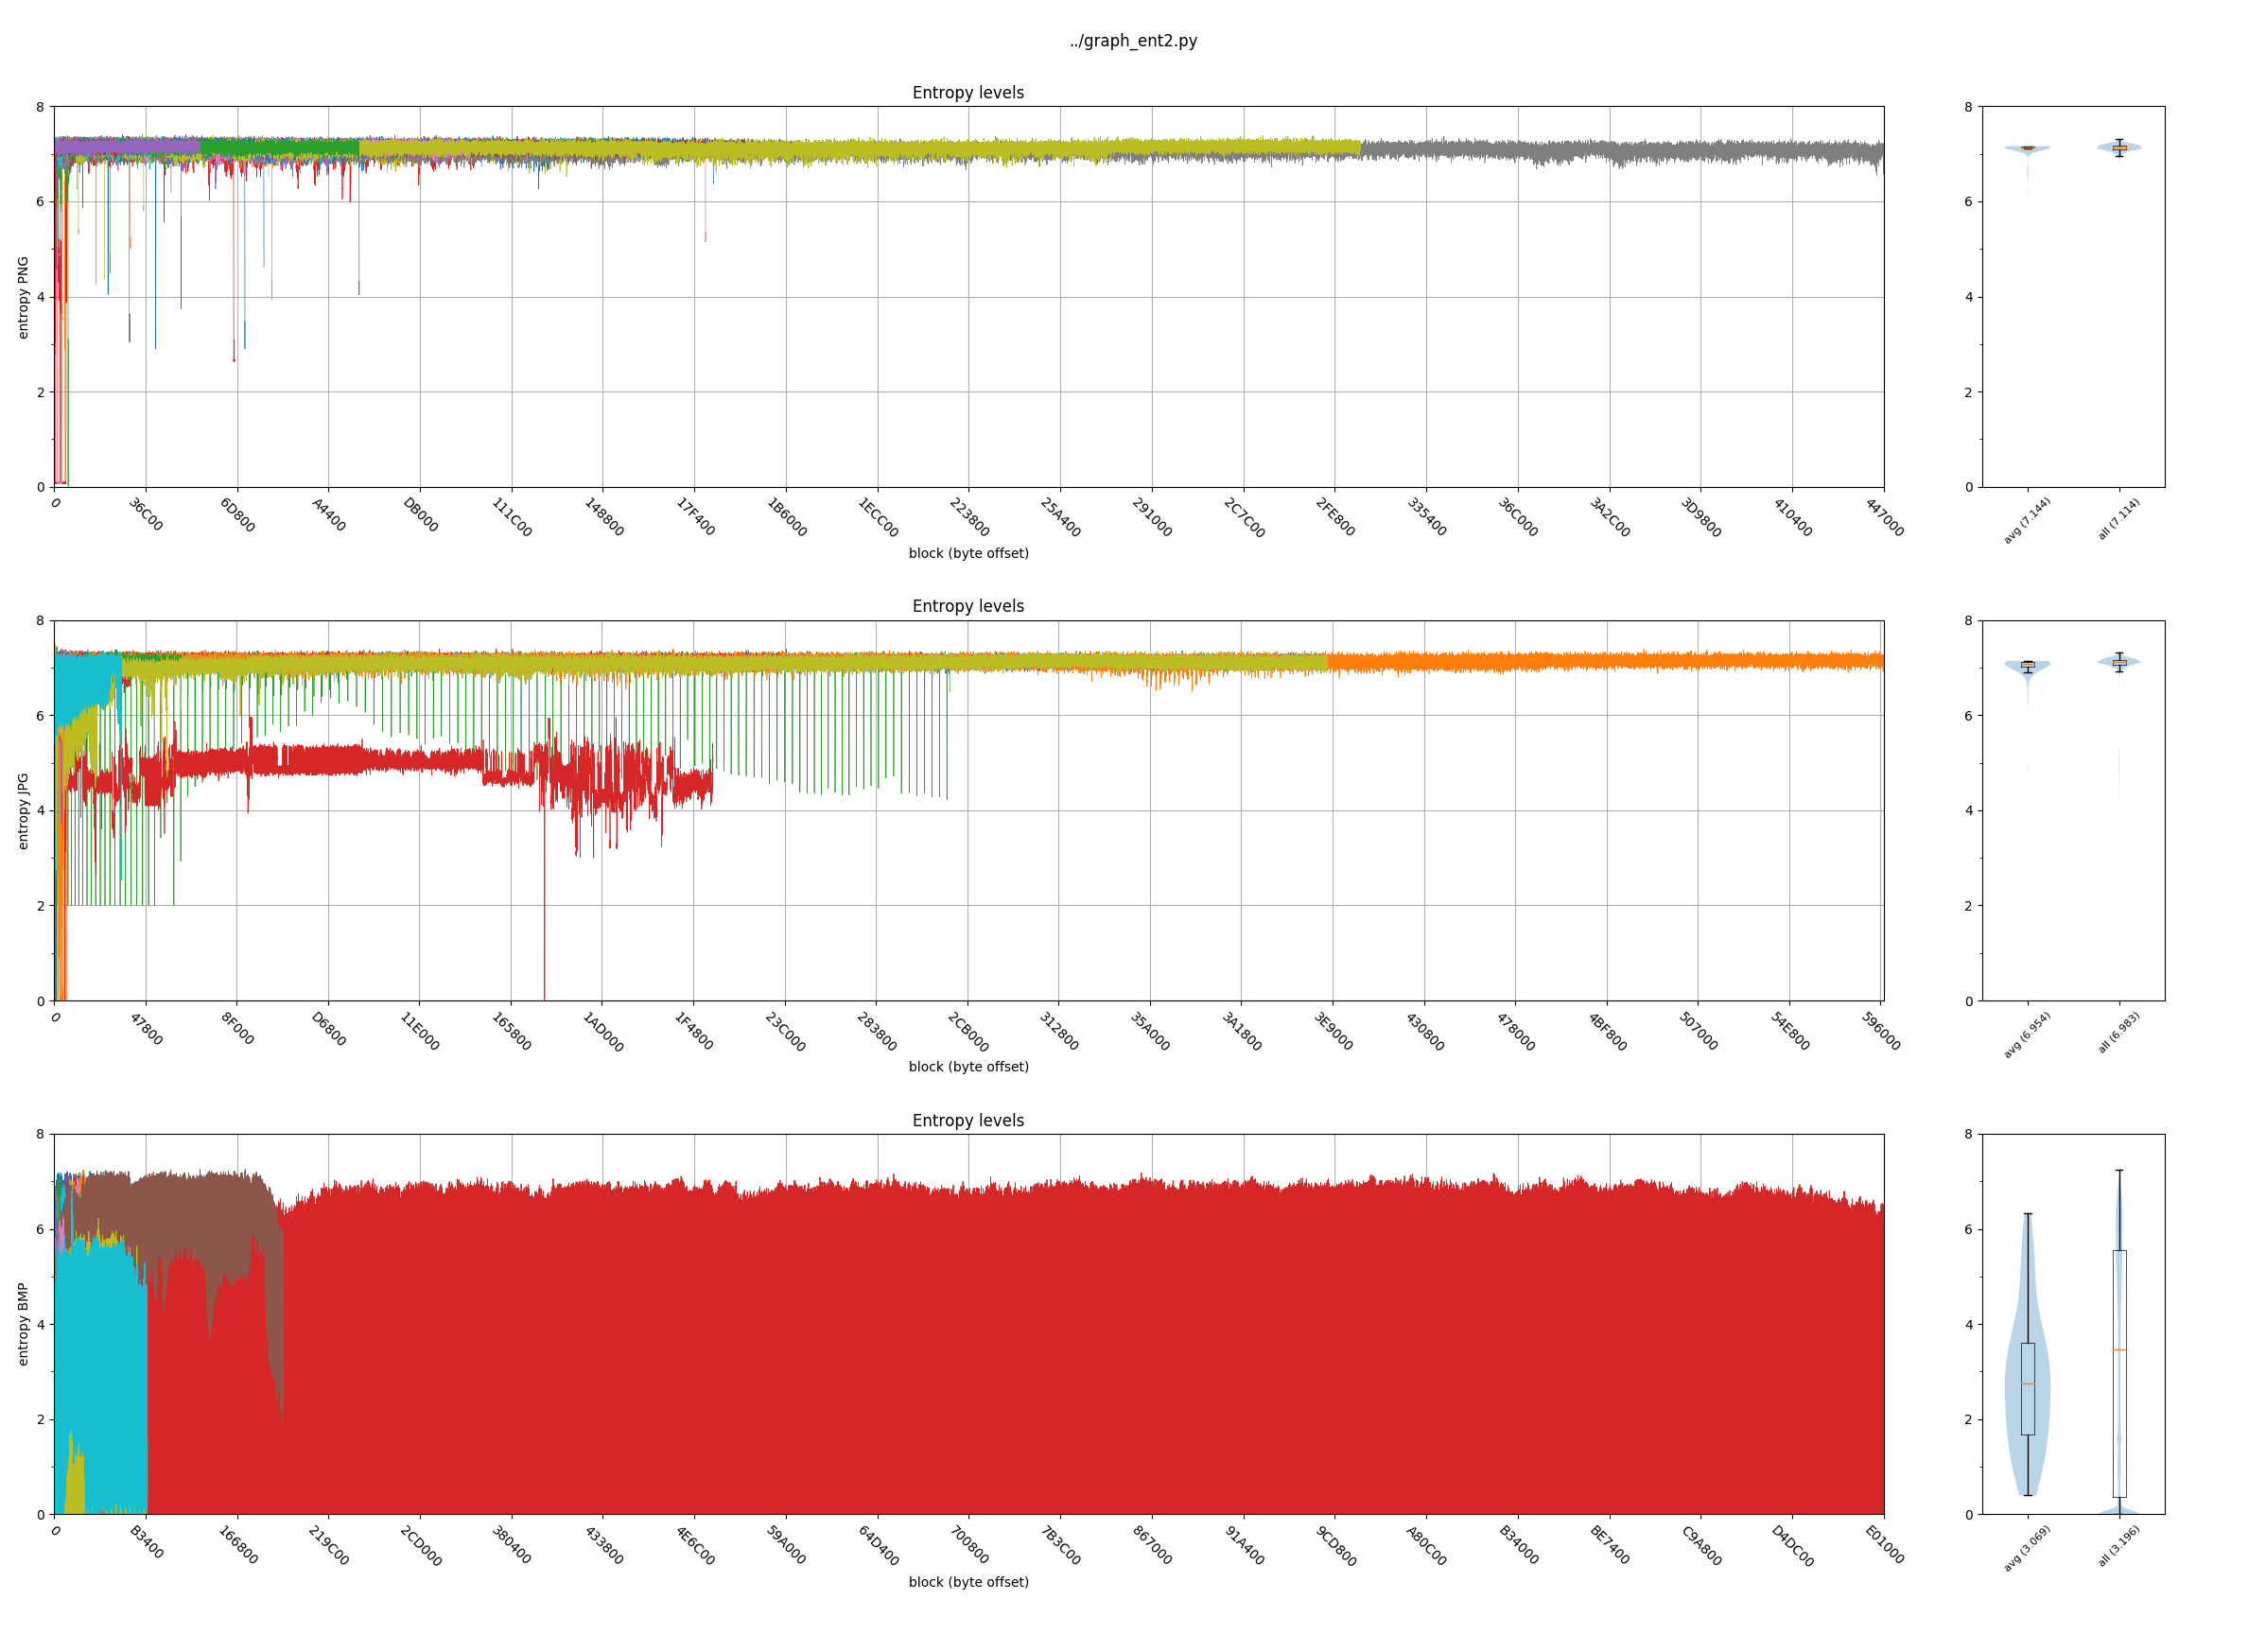
\includegraphics[width=\textwidth]{inc/statanalysis_graph}
	\caption{Distribution Analysis of Different, Common Graphics Formats}
	\label{fig:statGraph}
\end{figure*}

\begin{figure*}[ht]
	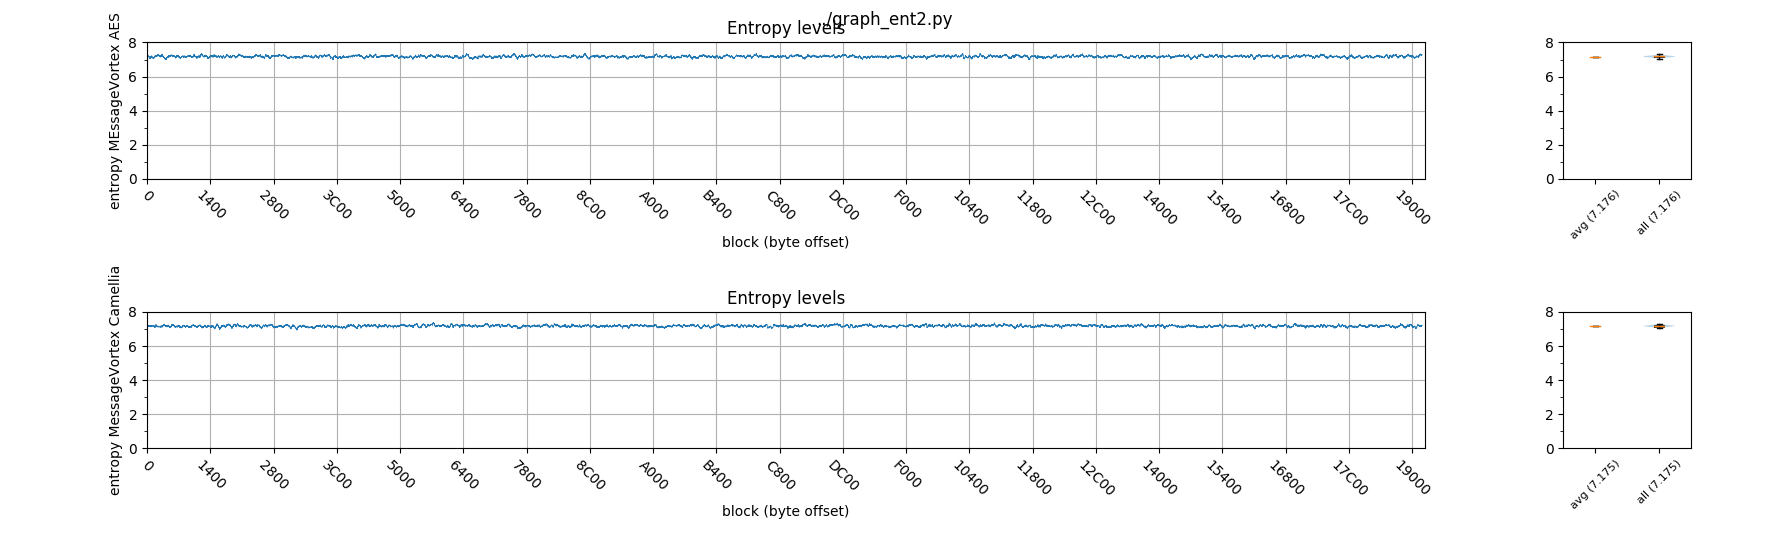
\includegraphics[width=\textwidth]{inc/statanalysis_mv}
	\caption{Distribution analysis of a MessageVortex block}
	\label{fig:statMvGraph}
\end{figure*}

We then carried out an analysis identifying the typical entropy and the inner structures. The graphs in \cref{fig:statGraph} show a typical analysis. In that specific case, we looked at 100 images of each type. We graphed and analyzed their entropy and tested for the suitability of a plain embedding from an entropy poi. Table~\ref{tab:fileEntropy} lists the average entropy of analyzed file types and makes remarks about the suitability for plain embedding. In practice, we found that most suitable file formats have an entropy of $\approx 7.2$ and an interquartile range (IQR) of 0.15 or less. Furthermore, files should have a big, uniform, non-structured range of octets containing these characteristics. Such a file has a suitable space for embedding. For reference, \cref{fig:statMvGraph} shows the distribution of typical \MessageVortex{} blocks. We did find that the entropy must be uniformly matched in the case of plain embedding.

\begin{table*}[!ht]
	\centering\tiny
	\begin{tabular}{|l|l|l|l|}\hline
		\diaghead{\theadfont Type Criteria}{Type}{Criteria} & \thead{Avg. Entropy}     & \thead{IQR} & \thead{Remarks}\\\hline
		JPG       & 7.008  & 0.097 & -- \\              
		PNG       & 7.116  & 0.086 & -- \\              
		GIF       & 6.978  & 0.194 & -- \\              
		BMP       & 2.997  & 4.964 & not suitable \\              
		PDF       & 6.660  & 0.282 & Hard to embed due to a very complex inner structure but well suited \\\hline              
		MP3       & 7.076  & 0.091 & -- \\              
		WAV       & 4.777  & 0.927 & -- \\              
		OGG       & 7.104  & 0.093 & relatively easy to embedd. Hard not to break the file structure. \\\hline              
		mpg4      & n/a    & n/a   & good to embedd. Steganography could be applied here easily too. \\\hline              
		zip       & 7.148  & 0.080 & easy to embedd when using ``password protected''  archives \\\hline\hline
		MVaes     & 7.176  & 0.072 & Without length padding as reference encrypted with AES 256 CBC\\
		MVcam     & 7.175  & 0.070 & Without length padding as reference encrypted with Camellia 256 CBC\\\hline
	\end{tabular}    
	\caption{comparison of protocols in terms of the suitability criteria as transport layer}
	\label{tab:fileEntropy}
\end{table*}

When blending into images, BMP showed a strongly varying entropy within a file. A sampling of ten blocks at random position resulted already in detection with a false positive rate below 5\%. PNG and JPG files showed to be very robust within the sample. We did not succeed in identifying the \MessageVortex{} blending content based on entropy values. GIF images showed to be unsuitable. Archive formats such as zip files were extremely robust. We were able to embed it into a zip file and marking it (generically) as an encrypted file. This embedding was genuinely undetectable. However, such embedding may potentially lead to censorship based on the blacklisting of encrypted zip files.

OGG and MP3 are suitable. However, we were able to detect the entropy difference when taking extremely dense samples. These formats may, however, be suitable for not yet standardized forms of steganography. While PDF typically has low entropy and a high IQR, some parts of the files are very well suited for embedding. Plain embedding with knowledge of the format was even possible without affecting the visual result of the file.

We could show that with an approach based on Shannon entropy, we may identify plain embedded \VortexMessages{} in BMP and WAV files. 

All movie formats were performing similarly to jpg and PNG. However, due to the very complex structure with scattered blocks, they seem to be unsuitable for plain embedding. They are, however, strong candidates for steganography and are being used.

\section{Analysis of Routing Layer}
\subsection{Analysis of Core Operations}
The core operations form a toolset for mixing messages. Under the operational restrictions outlined in \cref{sec:routingStrategies}, we analyze in the following section the operations and determine their capability for leaking information or affecting security.

\subsubsection{Splitting and Merging}
The operations $splitPayload$ and $mergePayload$ are the trivial operations of our operations set. The operations by themselves leak some information under the assumption that they were encrypted previously. A split or merge operation on its own leaks possible counterparts as the size should add up to a blocksize common in symmetric cryptography. As we outlined in \cref{sec:mergeAndSplit} and \cref{sec:routingStrategies} either an encryption step or an add redundancy step has to be added before a \VortexNode{} may forward the block to the next layer. When doing so, we can say that the operation leaks not more than any cryptographically secure operation.

For a \VortexNode{} executing the operation, a split operation does not leak any additional properties. The input may be payload or not. Therefore, the output of the operation has the same properties as the input. Unless the \VortexNodes{} knows the incoming payload's nature, the output may be either decoy or true message traffic.

\subsubsection{Encryption and Decryption Operations}
All encryption steps leak some properties. They may leak the algorithm due to the block size. The chosen parameter may be unique to the RBB. If randomly chosen, this is no longer the case. If chosen by an implementation-specific pattern, the pattern may leak the implementation over time. As the analysis must be done over a short period (the lifetime of an \defref{eID}), it is up to an RBB to leak as little information as possible. However, we regard the cryptographically secured content as secure. 

\subsubsection{Add and Remove Redundancy Operations}\label{sec:analysisReedSolomon}
During analysis, the $addRedundancy$ operation showed the undesirable behavior that applying the operation lowered the target blocks' entropy, as shown in \cref{fig:entropy}. 

Thus, we reconsidered the whole operation. The choice of the Reed--Solomon (RS) operation instead of a Lagrange polynomial seemed logical. As the possibilities to recover from cheaters in an RS setting of varying contexts have already been studied in~\cite{mceliece1981sharing},~\cite{bu2017rasss}, and similar publications.

%%%%%%%%%%%%%%%%%%%%%%%%%%%%%%%
%%% Preplaced float
%%%%%%%%%%%%%%%%%%%%%%%%%%%%%%%
\begin{figure*}[!t]\centering
	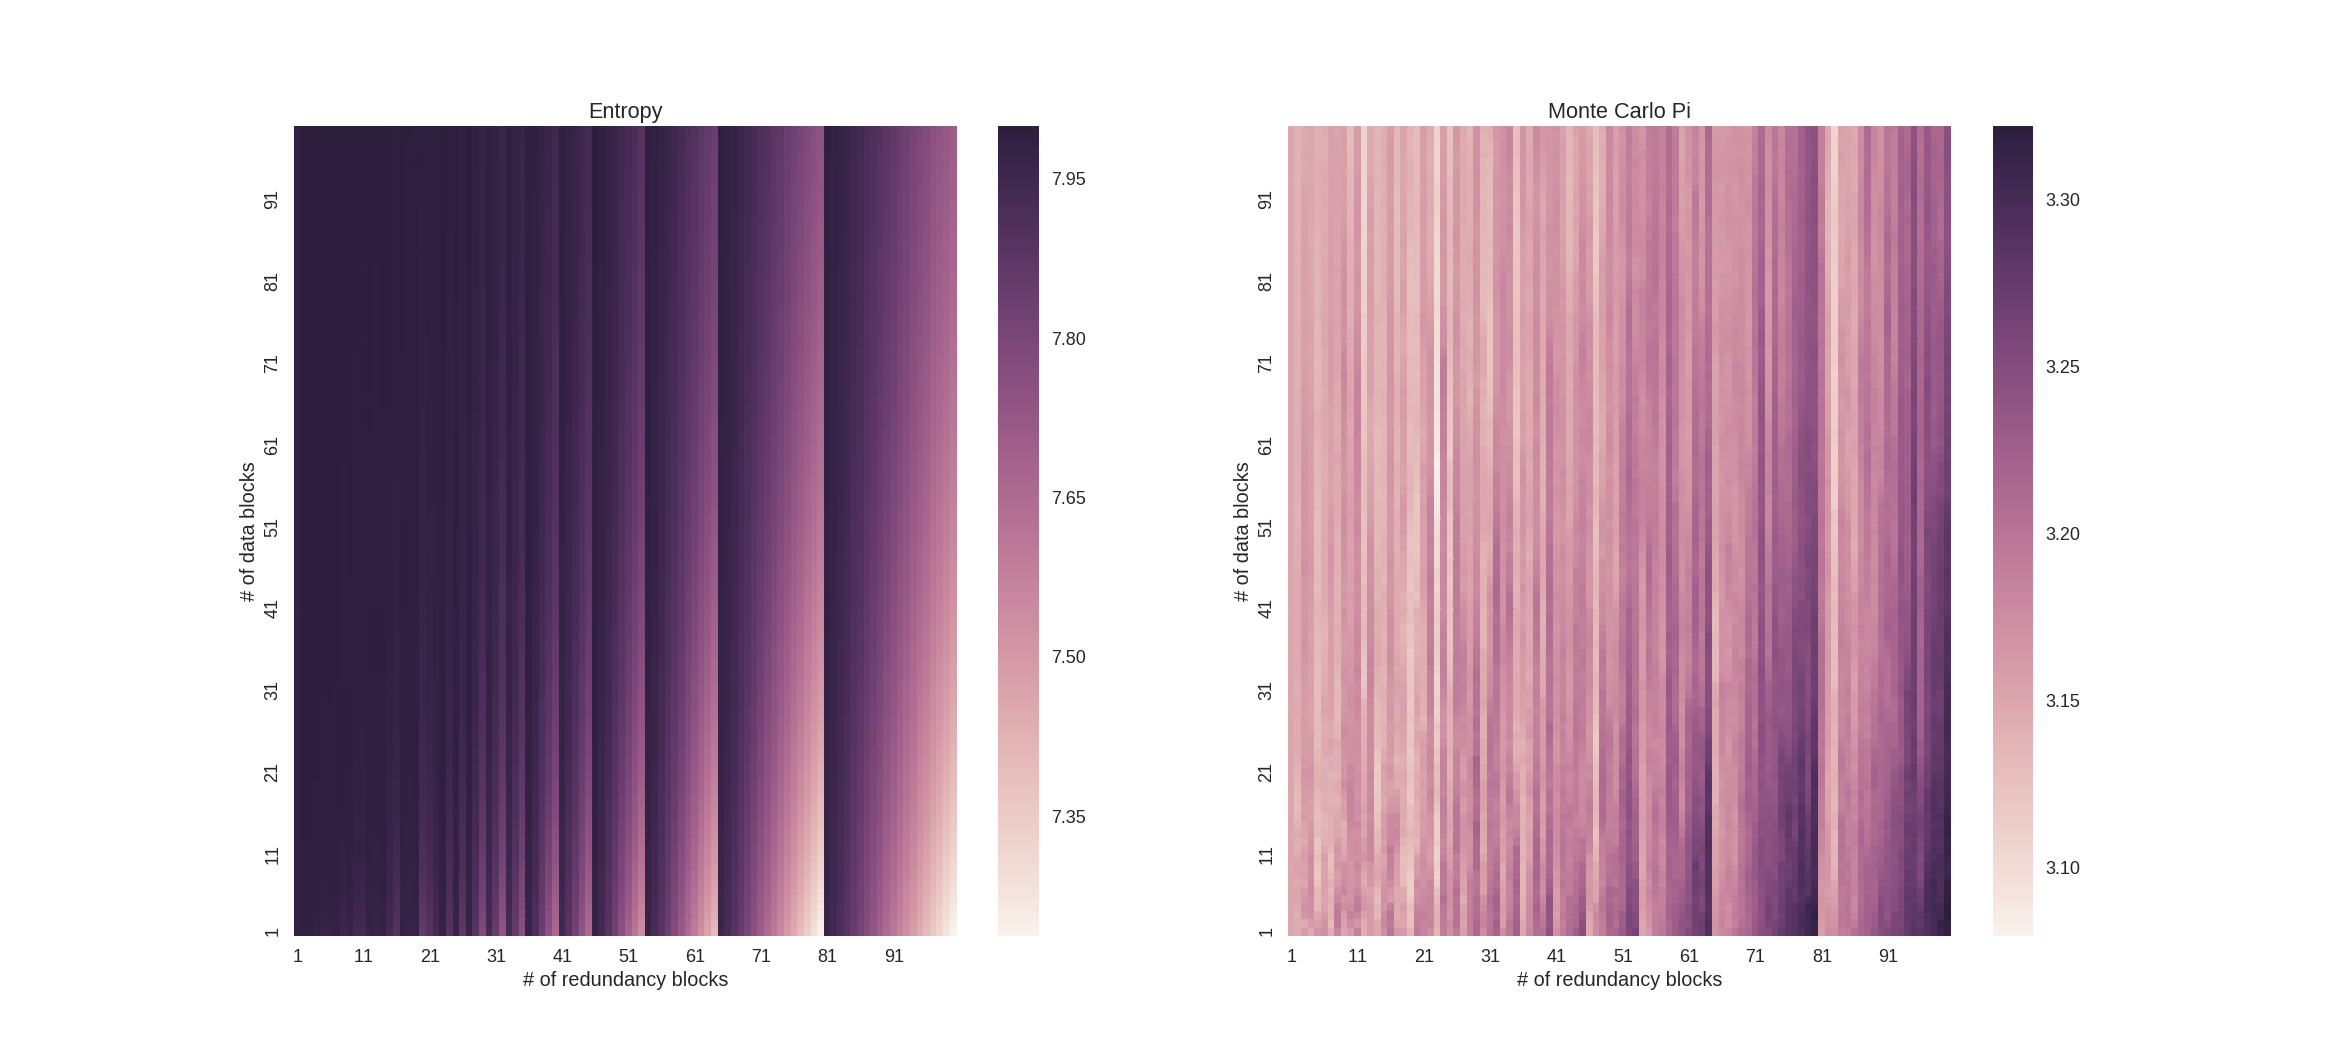
\includegraphics[width=1\textwidth]{inc/randomblock_10kb}
	\caption{Resulting entropy of addRedundancy with and without encryption step}
	\label{fig:entropy}
\end{figure*}


\section{Knowledge of a Node Sending the First Message}
A sender of a \VortexMessage{}, which is not equal to the RBB, may have knowledge about the initial routing block size and, therefore, guess the routing path's complexity. He is, however, unable to gain any additional information such as time of travel or number of hops until the target is reached. The building instructions  only leak minimal information which may also include some ideas about the routing block's complexity. 

As with every routing node, the next hops are leaked to the sender. Again this is done without leaking the next-hops host key.

\section{Intermediate Node Routing Layer}
An intermediate node knows all the operations applied and the immediate next hop. It learns the routing addresses of the immediately following endpoints but is unable to use these endpoints. This inability is based on the fact that the node has no means to obtain the host key required to communicate.

If a routing block is repeated, a router may identify the routing block as repetition. Identifying the repetition of a block can be achieved by looking at the serial number of replay protection. We then may give a rough estimate of the message size by comparing the payload chunks. However, this estimate is very rough as it is bounded by the block size of the symmetrically applied encryption.

\section{Security of Protocol Blocks}
To analyze the security of the protocol, we first go through all protocol blocks. Then we will look at the possibilities of block recombinations and how to gain data or services based on such behavior. 

Assuming plain embedding, the presence of a chain of blocks may leak an existing \VortexMessage. Currently, the protocol expects at the blending offset size and number of the bytes to be skipped to the next block. The encoding does not assume an end of the chain marker as such a marker would make the design identifiable. As an encoding scheme, a variable byte length has been chosen. This variable byte length guarantees that any file will always result in a valid chain of blocks and thus not leak such a presence.

The entropy of the only two blocks in this stream (MPREFIX and InnerMessageBlock) is comparable as both blocks are encrypted. Both blocks are encrypted and feature a similar entropy. The blocks follow each other without any delimiter. This results in a continuous stream of data with constant properties. 

To avoid repeating patterns at the beginning of streams due to reused identity blocks, a MURB must provide sufficient peer keys and prefix blocks. However, a \VortexNode{} may refuse to process MURBs (only accept maxReplays equal to 0).

All blocks of the InnerMessageBlock are protected by the peer key $E^{K_{peer}}$. The forward secrets in all blocks except the payload blocks ensure that the recombination of blocks does not work for an adversary. To be successful, an adversary requires to know the forward secret of the next hop.

To keep the secrets of the next node hidden from the host assembling the message, the subsequent header and the routing block are protected by the sender key $E^{K_{sender}}$. A message assembling node is thus not even capable of creating its own messages to an unknown node as the hosts' public key $E^{K^{1}_{host}}$ is not derivable from a message.

Therefore, a routing node cannot assemble messages for a specific host on the base of a routed message only. A routing node does not gain any additional knowledge except for the locally executed operations, the number of messages of the ephemeral identity, the size of messages of any ephemeral identity, the sending IP of a received \VortexMessage, and the transport endpoint address of any receiving endpoint. The most critical information is endpoint data, as all other data is unrelated to the original message (sender recipient and size). This information becomes crucial if assuming a censoring adversary. Therefore, a sender in a jurisdiction where MessageVortex{} is deemed illegal must use only trusted nodes within the jurisdiction and at least for the first hop outside the jurisdictional reach of an adversary.


\chapter{Dynamic Attack Analysis}\label{sec:dynamicAnalysis}
In the dynamic analysis, we reach out to an active adversary. An active adversary modifies traffic in a non-protocol conforming way or misuses available or obtained information to disrupt messages, nodes, or the system as a whole.

\section{Well-Known Attacks}\label{sec:wellKnownAttacks}
In the following sections, we emphasize on possible attacks to anonymity preserving protocols. Such attacks may be used to attack the anonymity of any entity involved in the message channel. In a later stage, we test the protocol for immunity against these classes of attacks.

\subsection{Broken Encryption Algorithms}
Encryption algorithms can become broken at any time. Our protocol is especially susceptible to this as it offers no perfect forward secrecy (PFS) on the transport layer. This either to new findings in attacking them, by more resources being available to an adversary, or by new technologies allowing new kinds of attacks. A proper protocol must be able to react to such threats promptly. This reaction should not rely on a required update of the infrastructure. Users should solely control the grade of security. 

We cannot wholly prevent such attacks from happening. However, we can introduce a choice of algorithms, paddings, modes, and key sizes to give the user a choice in the degree of security he wants to have.

We introduced a way to support a set of independent cryptographic algorithms, paddings, modes, and prngs. The support of these algorithms does not have to be uniform throughout the system. Instead, it is sufficient for two neighboring nodes to support the same algorithms in order to be used. 

Another way of minimizing the impact of reduced security of encryption algorithms is to use long host keys. If an algorithm's security is only reduced by a couple of bits instead of being broken, then a long key minimizes the impact and ay buy some time to switch to an alternate algorithm. 

A broken algorithm is severe if it leads to the decryption of the final messages on the recipient node. In such a case, an adversary would be able to rebuild the content of a workspace and thus effectively enable the adversary to obtain the message's content.

\subsection{Attacks Targeting Anonymity}
Attacks targeting users' anonymity are the main focus of this work. Many pieces of information can be leaked, and the primary goal should rely on the principles established in security.

\begin{itemize}
	\item Preventing an attack\\
	Attack prevention can only be achieved for attacks that are already known and thus may not be realistic in all cases. In our protocol, we have strict boundaries defined. A node under attack should at any time of protocol usage (this excepts bandwidth depletion attacks) be able to block malicious identities. Since establishing new identities is costly for an attacker, he should always require far more resources than the defender.
	\item Minimizing the attack surface\\
	This part of the attack prevention is included by design in the protocol. By minimizing the information footprint we have in each operation and the disconnection between two \defref{eID}s of the same sender, it is very difficult to gain additional information based on statistical means.
	\item Redirecting an attack\\
	Although the implementation does not do this, it is possible to handle suspected malicious \VortexNode{} differently (e.g., avoid using them or only use them for decoy traffic, not disclosing identities).
	\item Controlling damage\\
	For us, this means leaving as little information about identities or meta information as possible on untrusted infrastructures. If we leave traces (i.e., message flows or accounting information), they should have the least possible information content and expire within a reasonable amount of time.
	\item Discoveruing an attack\\
	The protocol is designed, so that attack discovery (such as a query attack) is possible. However, we consider active attacks just as part of the regular message flow. The protocol must mitigate such attacks by design.
	\item Recovering from an attack\\
	An attack does always impose a load onto a system's resources, regardless of its success. It is vital that a system recovers almost immediately from an attack and is not covered in a non-functional or only partially functional state either temporarily or permanently.
\end{itemize}

In the following subsections, we list a couple of attack classes that have been used against systems listed in \cref{sec:implSystems} or the respective academic works. We list the countermeasures which have been taken to deflect these attacks.

\subsubsection{Probing Attacks}
Identifying a node by probing and check their reaction is commonly done when fingerprinting a service. As a node is participating in a network and relaying messages probing may not be evaded. However, it may be made costly for an adversary to do systematic probing. This should be taken into account. Both currently specified transport protocols feature an indefinite number of possible accounts. Since not the server but the endpoint address is behaving, node probing is more complicated than in other cases where probing of service is sufficient. 

One of the problems is cleartext requests. These requests may be used on any transport layer account without previous knowledge of any host key. Thus the recommendation in \cref{tab:protoReplyCrit} is generally not to answer the requests. Routing nodes in jurisdictions not fearing legal repression or prosecution may reply to cleartext requests, but it is usually discouraged as they allow harvesting of \VortexNodes{}. A discovered \VortexNode{} may leak subsequent nodes if the same account is used for receiving and sending.

%FIXME2: is that statement really true or just delaying? Hi cost=high CPU consumption-> long reply time
One strategy to avoid this would be to put high costs onto cleartext requests so that a cleartext request may have a long reply time (e.g., up to one day). 

A node is free to blacklist an identity in case of an early reply. This is an insufficient strategy as a big adversary may have lots of identities in stock. Requesting an unusually long key as a plaintext identity does not make sense either, as these as well may be kept in stock. However, we may force a plaintext request to have an identity block with a hash following specific rules. For example, we may put in a requirement that the first four bytes of the hash of a header block correspond to the first four characters of the routing block. At the moment, this has been rejected in the standard for practical reasons. First, as the request is unsolicited, a sender is the only one able to decide the hash's algorithm. This would allow a requester to choose upon the complexity of the puzzle. Second, any negotiation of the request's cost would result in the disclosure of the node as \VortexNode, which might be unsuitable.

\subsubsection{Hotspot Attacks}
Hotspot attacks aim to isolate high traffic sites within a network. By analyzing specific properties or the general throughput locations with outstanding traffic may be identified. These messages do quite often reveal senders or recipients. Sometimes an intermediate node in an anonymizing system. 

The assumption that a hotspot arises at a specific point in our protocol is wrong. At any point in the lifecycle of a message, either payload blocks are left out until expiry, or additional traffic may be generated using an $addRedundancy$ operation.

\subsubsection{Message Tagging and Tracing}
When using an anonymization system, a message may be either fully or partially traced or even tagged. Tagging allows one to recognize a message at a later stage and map it to its predecessors. Protocols with tagable messages are not suitable for anonymization systems.

\VortexMessages{} are not tagable. The constraint ``no repeating pattern'' prohibits forwarding of any block without an appropriate operation. This denies the possibility of tagging a payload block. All other blocks (prefixes, header, and routing block) are discarded when forwarding the message. The same applies to the carrier message, which is used as transport for the blended \VortexMessage.

Injecting a value into a payload block and following it would imply that the evil \VortexNode{} has knowledge about all subsequent operations and keys, which is equivalent to know the subsequent private keys of the \VortexNodes. We will cover this scenario in \cref{sec:analysisInteractionGraphs}.

\subsubsection{Side Channel Attacks}
Side-channel attacks are numerous. Especially important to us are attacks related to either lookup in independent channels (e.g., downloading of auxiliary content of a message) or behavior related to timing patterns.

\subsubsection{Sizing Attacks}
There are two types of sizing attacks identified as relevant for us. One is the possibility of matching messages with related sizes, and the other is to relate message size to the original messages. Both attacks may be considered as a tracing attack and will be analyzed accordingly. 

When matching messages in size, an attack is attractive if it allows collapsing the operations of one or multiple honest \VortexNodes{} between two malicious \VortexNodes. To do so, the second evil node may match the sizes of the received payload blocks and hypothesize about which blocks are equal, or it may assign the \defref{eID} of the first evil node to the \defref{eID} of the second node. The matching is not trivial, as\ldots

\begin{enumerate}
	\item The sizes are likely to have changed while transferred through the honest nodes.
	\item The number of payload blocks may have changed.
	\item The size may have been further obfuscated because an onionized encryption does either not add to the size (if an algorithm with the same block size is applied and no padding) or is increasing (by the block size). Obfuscation is possible as well, if we apply a $splitPayload$ or $mergePayload$ operation with a subsequent encryption (mandatory to not violate the ``repeating pattern rule'') or an $addRedundancy$ operation.
\end{enumerate}

\subsubsection{Bugging Attacks}
Numerous attacks are available through the bugging of a protocol. In this chapter, we outline some of the possibilities and how they may be countered:

\begin{itemize}
	\item Bugging through certificate or identity lookup:\\
	Almost all types of proof of identitie, such as certificates, offer some revocation facility. While this is a perfect desirable property of these infrastructures, they have a flaw. Since the location of this revocation information is typically embedded in the proof of identity, an evil attacker might use a falsified proof of identity with a recording revocation point.
	
	There are multiple possibilities to counter such an attack. The easiest one is to do no verification at all. Having no verification is, however, not desirable from the security point of view. Another possibility is only to verify trusted proof of identities. By doing so, the only attacker could be someone having access to a trusted source of proof of identities. A third possibility is relaying the request to another host either by using an anonymity structure such as Tor or using its infrastructure. Using Tor would violate the ``Zero Trust'' goal. Such a measure would only conceal the source of the verification. It would not hide the fact that the message is processed. A fourth and most promising technology would be to force the sender of the certificate to include a ``proof of non-revocation''. Such proof could be a timestamped and signed partial CRL. It would allow a node to verify a certificate's validity without being forced to disclose itself by doing a verification. On the downside, including a proof of non-revocation involves the requirement to accept a certain amount of caching time to be accepted. This caching cycle reduces the value of the proof as it may be expired in the meantime. It is recommended to keep the maximum cache time as low as 1d to avoid that revoked certificates may be used. 
	
	\item Bugging through DNS traffic:\\
	A standard protocol on the Internet is DNS. Almost all network-related programs use it without considering effects on anonymity. %FIXME2 Reworded
	 Typically, the use of such protocol is only a minor issue since an ISP usually makes the resolution of a lookup. Normally an ISP would not keep a query log as such logs tend to become big, and their information content is comparatively low. In the case of a censoring adversary, an ISP may be forced to keep such a log or to provide access to the adversary.
	
	The bugging in general attack works as follows: We include a unique DNS name to be resolved by a recipient. This can be done most easily by adding an external resource such as an image. A recipient will process this resource and might therefore deliver information about the frequency of reading or the type of client. 
	
	It must be taken into account that the transport layer will always do DNS lookups and that we may not avoid this attack completely. We may, however, minimize the possibilities of this attack.
	
	\item Bugging through external resources:\\
	A straightforward attack is always to include external resources into a message and wait until they are fetched. In order to avoid this kind of attack, plain text or other self-contained formats should be used when sending a message. As we may not govern the type of contained message, we can make at least recommendations concerning its structure.
\end{itemize}

\subsubsection{Analysis by Building Interaction Graphs\label{sec:analysisInteractionGraphs}}
Building interaction graphs is very hard with our system. Although we cannot quantize the effect, we still may elaborate on the difficulties. We first look at our system from an outside view and then do the same for a powerful adversary inside the system.

When looking from outside the system, interaction graphs are hard to build as sending and receiving transport addresses, and protocols do not match, which adds tremendously to the complexity. An outside observer may not just observe a specific SMTP server. He must track incoming messages, observe the user (typically obtaining the mail by IMAP) fetching the messages, and then follow all possible connections to other infrastructures known to be supported and suspect them as outbound messages. By assuming that an outside observer is able to identify all \VortexMessages{} and surpass all difficulties involved in following the different protocols. Then such an observer is capable of generating a graph having as nodes all \VortexNodes{} and as edges all \VortexMessages{}. An adversary would then require the means to identify the sender and recipient. We first claim that there is no possibility to identify such senders and recipients as there is no guaranteed minimum or maximum time for a message. As an immediate result, any \VortexNode{} sending a message may be a sender of a message or only a router. Inversely, any \VortexNode{} receiving a message may be either a recipient or a router. Due to the operations, sizes may increase or decrease on message paths. Therefore, an outside adversary is unable to match two adjacent messages to the same identity. Any previous message, including all subsequent messages, may have triggered the sending of the message. So from an outside perspective, we have no possibility to identify by message pattern, message size, or message sequence adjacent messages.

We assume the example routing graph, as shown in \cref{fig:messageGraphPaths}.

\begin{figure*}[!t]\centering
	\resizebox{.9\linewidth}{!}{
		\begin{tikzpicture}		
	\tikzset{
		rounded/.style={rounded corners=3pt},	
		shadowed/.style={general shadow={fill=nodeshadow,shadow xshift=\shadowshift,shadow yshift=\shadowshift}},
 		hexnode/.style={regular polygon,regular polygon sides=6,draw,fill=operationcolor,inner sep=0mm,minimum size=2mm]},
		astyle/.style={-{Latex[length=2.5mm,width=1.5mm]},semithick},
		knode/.style={rectangle,fill=nodecolor,draw=black,thick,inner sep=8pt,baseline=(current bounding box.center),shadowed,rounded},
		nodestyle/.style={fill=nodecolor,rounded,anchor=center,shadowed},
		main/.style={draw,minimum width=0.5cm},child/.style={draw,minimum width=0.5cm},
	}
	%\tikzstyle{level 1}=[sibling angle=25.71]
	%\path(0,1000);
	\node[main] (a) {
		\begin{tikzpicture}
			\draw [nodestyle,fill=startnodecolor] (0,0) rectangle +(0.4,0.45) node[pos=.5] (n0) {0};
			\draw[nodestyle,fill=endnodecolor] (1.5,0) rectangle +(0.4,0.45) node[pos=0.5] (n1) {1};
			\draw[nodestyle] (3,0) rectangle +(0.4,0.45) node[pos=0.5] (n2) {2};
			\draw[nodestyle] (4.5,0) rectangle +(0.4,0.45) node[pos=0.5] (n3) {3};
			\draw[nodestyle] (6,0) rectangle +(0.4,0.45) node[pos=0.5] (n4) {4};
			\draw[nodestyle] (7.5,0) rectangle +(0.4,0.45) node[pos=0.5] (n5) {5};
			\draw[nodestyle] (9,0) rectangle +(0.4,0.45) node[pos=0.5] (n6) {6};
			\node[left = 0mm of n0] (nm0) {};
			\node[below of=n0, node distance=5cm] (n0Ground) {};
			\node[below of=n1, node distance=5cm] (n1Ground) {};
			\node[below of=n2, node distance=5cm] (n2Ground) {};
			\node[below of=n3, node distance=5cm] (n3Ground) {};
			\node[below of=n4, node distance=5cm] (n4Ground) {};
			\node[below of=n5, node distance=5cm] (n5Ground) {};
			\node[below of=n6, node distance=5cm] (n6Ground) {};
			\node[below of=nm0,node distance=5cm] (nm0Ground) {};
			% lines down
			\draw (n0) -- (n0Ground);
			\draw (n1) -- (n1Ground);
			\draw (n2) -- (n2Ground);
			\draw (n3) -- (n3Ground);
			\draw (n4) -- (n4Ground);
			\draw (n5) -- (n5Ground);
			\draw (n6) -- (n6Ground);
			%arrows
			\draw[astyle] ($(n0)!0.10!(n0Ground)$)--($(n1)!0.10!(n1Ground)$);
			\draw[astyle] ($(n0)!0.15!(n0Ground)$)--($(n3)!0.15!(n3Ground)$);
			\draw[astyle] ($(n1)!0.20!(n1Ground)$)--($(n2)!0.20!(n2Ground)$);
			\draw[astyle] ($(n0)!0.25!(n0Ground)$)--($(n1)!0.25!(n1Ground)$);
			\draw[astyle] ($(n3)!0.30!(n3Ground)$)--($(n4)!0.30!(n4Ground)$);
			\draw[astyle] ($(n0)!0.35!(n0Ground)$)--($(n3)!0.35!(n3Ground)$);
			\draw[astyle] ($(n3)!0.40!(n3Ground)$)--($(n5)!0.40!(n5Ground)$);
			\draw[astyle] ($(n0)!0.45!(n0Ground)$)--($(n6)!0.45!(n6Ground)$);
			\draw[astyle] ($(n3)!0.50!(n3Ground)$)--($(n1)!0.50!(n1Ground)$);
			\draw[astyle] ($(n5)!0.55!(n5Ground)$)--($(n1)!0.55!(n1Ground)$);
			\draw[astyle] ($(n3)!0.60!(n3Ground)$)--($(n0)!0.60!(n0Ground)$);
			\draw[astyle] ($(n5)!0.65!(n5Ground)$)--($(n0)!0.65!(n0Ground)$);
			\draw[astyle] ($(n6)!0.70!(n6Ground)$)--($(n4)!0.70!(n4Ground)$);
			\draw[astyle] ($(n5)!0.75!(n5Ground)$)--($(n0)!0.75!(n0Ground)$);
			\draw[astyle] ($(n2)!0.80!(n2Ground)$)--($(n6)!0.80!(n6Ground)$);
			\draw[astyle] ($(n3)!0.85!(n3Ground)$)--($(n2)!0.85!(n2Ground)$);
			\draw[astyle] ($(n2)!0.90!(n2Ground)$)--($(n5)!0.90!(n5Ground)$);
		\end{tikzpicture}
	} ;
	\node (1) at ($(a)+(-90+0*180/5:12.6cm) $) [child] {
		\begin{tikzpicture}
			\draw [nodestyle,fill=startnodecolor] (0,0) rectangle +(0.4,0.45) node[pos=.5] (n0) {0};
			\draw[nodestyle,fill=endnodecolor] (1.5,0) rectangle +(0.4,0.45) node[pos=0.5] (n1) {1};
			\draw[nodestyle] (3,0) rectangle +(0.4,0.45) node[pos=0.5] (n2) {2};
			\draw[nodestyle] (4.5,0) rectangle +(0.4,0.45) node[pos=0.5] (n3) {3};
			\draw[nodestyle] (6,0) rectangle +(0.4,0.45) node[pos=0.5] (n4) {4};
			\draw[nodestyle] (7.5,0) rectangle +(0.4,0.45) node[pos=0.5] (n5) {5};
			\draw[nodestyle] (9,0) rectangle +(0.4,0.45) node[pos=0.5] (n6) {6};
			\node[left = 0mm of n0] (nm0) {};
			\node[below of=n0, node distance=5cm] (n0Ground) {};
			\node[below of=n1, node distance=5cm] (n1Ground) {};
			\node[below of=n2, node distance=5cm] (n2Ground) {};
			\node[below of=n3, node distance=5cm] (n3Ground) {};
			\node[below of=n4, node distance=5cm] (n4Ground) {};
			\node[below of=n5, node distance=5cm] (n5Ground) {};
			\node[below of=n6, node distance=5cm] (n6Ground) {};
			\node[below of=nm0,node distance=5cm] (nm0Ground) {};
			% lines down
			\draw (n0) -- (n0Ground);
			\draw (n1) -- (n1Ground);
			\draw (n2) -- (n2Ground);
			\draw (n3) -- (n3Ground);
			\draw (n4) -- (n4Ground);
			\draw (n5) -- (n5Ground);
			\draw (n6) -- (n6Ground);
			%arrows
			\draw[astyle,thick,color=green] ($(n0)!0.10!(n0Ground)$)--($(n1)!0.10!(n1Ground)$);
			\draw[astyle] ($(n0)!0.15!(n0Ground)$)--($(n3)!0.15!(n3Ground)$);
			\draw[astyle] ($(n1)!0.20!(n1Ground)$)--($(n2)!0.20!(n2Ground)$);
			\draw[astyle] ($(n0)!0.25!(n0Ground)$)--($(n1)!0.25!(n1Ground)$);
			\draw[astyle] ($(n3)!0.30!(n3Ground)$)--($(n4)!0.30!(n4Ground)$);
			\draw[astyle] ($(n0)!0.35!(n0Ground)$)--($(n3)!0.35!(n3Ground)$);
			\draw[astyle] ($(n3)!0.40!(n3Ground)$)--($(n5)!0.40!(n5Ground)$);
			\draw[astyle] ($(n0)!0.45!(n0Ground)$)--($(n6)!0.45!(n6Ground)$);
			\draw[astyle] ($(n3)!0.50!(n3Ground)$)--($(n1)!0.50!(n1Ground)$);
			\draw[astyle] ($(n5)!0.55!(n5Ground)$)--($(n1)!0.55!(n1Ground)$);
			\draw[astyle] ($(n3)!0.60!(n3Ground)$)--($(n0)!0.60!(n0Ground)$);
			\draw[astyle] ($(n5)!0.65!(n5Ground)$)--($(n0)!0.65!(n0Ground)$);
			\draw[astyle] ($(n6)!0.70!(n6Ground)$)--($(n4)!0.70!(n4Ground)$);
			\draw[astyle] ($(n5)!0.75!(n5Ground)$)--($(n0)!0.75!(n0Ground)$);
			\draw[astyle] ($(n2)!0.80!(n2Ground)$)--($(n6)!0.80!(n6Ground)$);
			\draw[astyle] ($(n3)!0.85!(n3Ground)$)--($(n2)!0.85!(n2Ground)$);
			\draw[astyle] ($(n2)!0.90!(n2Ground)$)--($(n5)!0.90!(n5Ground)$);
		\end{tikzpicture}
	};
	\node (2) at ($(a)+(-84+1*180/5:17cm) $) [child] {
		\begin{tikzpicture}
			\draw [nodestyle,fill=startnodecolor] (0,0) rectangle +(0.4,0.45) node[pos=.5] (n0) {0};
			\draw[nodestyle,fill=endnodecolor] (1.5,0) rectangle +(0.4,0.45) node[pos=0.5] (n1) {1};
			\draw[nodestyle] (3,0) rectangle +(0.4,0.45) node[pos=0.5] (n2) {2};
			\draw[nodestyle] (4.5,0) rectangle +(0.4,0.45) node[pos=0.5] (n3) {3};
			\draw[nodestyle] (6,0) rectangle +(0.4,0.45) node[pos=0.5] (n4) {4};
			\draw[nodestyle] (7.5,0) rectangle +(0.4,0.45) node[pos=0.5] (n5) {5};
			\draw[nodestyle] (9,0) rectangle +(0.4,0.45) node[pos=0.5] (n6) {6};
			\node[left = 0mm of n0] (nm0) {};
			\node[below of=n0, node distance=5cm] (n0Ground) {};
			\node[below of=n1, node distance=5cm] (n1Ground) {};
			\node[below of=n2, node distance=5cm] (n2Ground) {};
			\node[below of=n3, node distance=5cm] (n3Ground) {};
			\node[below of=n4, node distance=5cm] (n4Ground) {};
			\node[below of=n5, node distance=5cm] (n5Ground) {};
			\node[below of=n6, node distance=5cm] (n6Ground) {};
			\node[below of=nm0,node distance=5cm] (nm0Ground) {};
			% lines down
			\draw (n0) -- (n0Ground);
			\draw (n1) -- (n1Ground);
			\draw (n2) -- (n2Ground);
			\draw (n3) -- (n3Ground);
			\draw (n4) -- (n4Ground);
			\draw (n5) -- (n5Ground);
			\draw (n6) -- (n6Ground);
			%arrows
			\draw[astyle] ($(n0)!0.10!(n0Ground)$)--($(n1)!0.10!(n1Ground)$);
			\draw[astyle,thick,color=green] ($(n0)!0.15!(n0Ground)$)--($(n3)!0.15!(n3Ground)$);
			\draw[astyle] ($(n1)!0.20!(n1Ground)$)--($(n2)!0.20!(n2Ground)$);
			\draw[astyle] ($(n0)!0.25!(n0Ground)$)--($(n1)!0.25!(n1Ground)$);
			\draw[astyle] ($(n3)!0.30!(n3Ground)$)--($(n4)!0.30!(n4Ground)$);
			\draw[astyle] ($(n0)!0.35!(n0Ground)$)--($(n3)!0.35!(n3Ground)$);
			\draw[astyle] ($(n3)!0.40!(n3Ground)$)--($(n5)!0.40!(n5Ground)$);
			\draw[astyle] ($(n0)!0.45!(n0Ground)$)--($(n6)!0.45!(n6Ground)$);
			\draw[astyle,thick,color=green] ($(n3)!0.50!(n3Ground)$)--($(n1)!0.50!(n1Ground)$);
			\draw[astyle] ($(n5)!0.55!(n5Ground)$)--($(n1)!0.55!(n1Ground)$);
			\draw[astyle] ($(n3)!0.60!(n3Ground)$)--($(n0)!0.60!(n0Ground)$);
			\draw[astyle] ($(n5)!0.65!(n5Ground)$)--($(n0)!0.65!(n0Ground)$);
			\draw[astyle] ($(n6)!0.70!(n6Ground)$)--($(n4)!0.70!(n4Ground)$);
			\draw[astyle] ($(n5)!0.75!(n5Ground)$)--($(n0)!0.75!(n0Ground)$);
			\draw[astyle] ($(n2)!0.80!(n2Ground)$)--($(n6)!0.80!(n6Ground)$);
			\draw[astyle] ($(n3)!0.85!(n3Ground)$)--($(n2)!0.85!(n2Ground)$);
			\draw[astyle] ($(n2)!0.90!(n2Ground)$)--($(n5)!0.90!(n5Ground)$);
			% addon arrows
			\draw[astyle,thick,color=green] ($(n3)!0.15!(n3Ground)$)--($(n3)!0.50!(n3Ground)$);
		\end{tikzpicture}
	};
	\node (3) at ($(a)+(-90+2*180/5:17cm) $) [child] {
		\begin{tikzpicture}
			\draw [nodestyle,fill=startnodecolor] (0,0) rectangle +(0.4,0.45) node[pos=.5] (n0) {0};
			\draw[nodestyle,fill=endnodecolor] (1.5,0) rectangle +(0.4,0.45) node[pos=0.5] (n1) {1};
			\draw[nodestyle] (3,0) rectangle +(0.4,0.45) node[pos=0.5] (n2) {2};
			\draw[nodestyle] (4.5,0) rectangle +(0.4,0.45) node[pos=0.5] (n3) {3};
			\draw[nodestyle] (6,0) rectangle +(0.4,0.45) node[pos=0.5] (n4) {4};
			\draw[nodestyle] (7.5,0) rectangle +(0.4,0.45) node[pos=0.5] (n5) {5};
			\draw[nodestyle] (9,0) rectangle +(0.4,0.45) node[pos=0.5] (n6) {6};
			\node[left = 0mm of n0] (nm0) {};
			\node[below of=n0, node distance=5cm] (n0Ground) {};
			\node[below of=n1, node distance=5cm] (n1Ground) {};
			\node[below of=n2, node distance=5cm] (n2Ground) {};
			\node[below of=n3, node distance=5cm] (n3Ground) {};
			\node[below of=n4, node distance=5cm] (n4Ground) {};
			\node[below of=n5, node distance=5cm] (n5Ground) {};
			\node[below of=n6, node distance=5cm] (n6Ground) {};
			\node[below of=nm0,node distance=5cm] (nm0Ground) {};
			% lines down
			\draw (n0) -- (n0Ground);
			\draw (n1) -- (n1Ground);
			\draw (n2) -- (n2Ground);
			\draw (n3) -- (n3Ground);
			\draw (n4) -- (n4Ground);
			\draw (n5) -- (n5Ground);
			\draw (n6) -- (n6Ground);
			%arrows
			\draw[astyle] ($(n0)!0.10!(n0Ground)$)--($(n1)!0.10!(n1Ground)$);
			\draw[astyle] ($(n0)!0.15!(n0Ground)$)--($(n3)!0.15!(n3Ground)$);
			\draw[astyle] ($(n1)!0.20!(n1Ground)$)--($(n2)!0.20!(n2Ground)$);
			\draw[astyle,thick,color=green] ($(n0)!0.25!(n0Ground)$)--($(n1)!0.25!(n1Ground)$);
			\draw[astyle] ($(n3)!0.30!(n3Ground)$)--($(n4)!0.30!(n4Ground)$);
			\draw[astyle] ($(n0)!0.35!(n0Ground)$)--($(n3)!0.35!(n3Ground)$);
			\draw[astyle] ($(n3)!0.40!(n3Ground)$)--($(n5)!0.40!(n5Ground)$);
			\draw[astyle] ($(n0)!0.45!(n0Ground)$)--($(n6)!0.45!(n6Ground)$);
			\draw[astyle] ($(n3)!0.50!(n3Ground)$)--($(n1)!0.50!(n1Ground)$);
			\draw[astyle] ($(n5)!0.55!(n5Ground)$)--($(n1)!0.55!(n1Ground)$);
			\draw[astyle] ($(n3)!0.60!(n3Ground)$)--($(n0)!0.60!(n0Ground)$);
			\draw[astyle] ($(n5)!0.65!(n5Ground)$)--($(n0)!0.65!(n0Ground)$);
			\draw[astyle] ($(n6)!0.70!(n6Ground)$)--($(n4)!0.70!(n4Ground)$);
			\draw[astyle] ($(n5)!0.75!(n5Ground)$)--($(n0)!0.75!(n0Ground)$);
			\draw[astyle] ($(n2)!0.80!(n2Ground)$)--($(n6)!0.80!(n6Ground)$);
			\draw[astyle] ($(n3)!0.85!(n3Ground)$)--($(n2)!0.85!(n2Ground)$);
			\draw[astyle] ($(n2)!0.90!(n2Ground)$)--($(n5)!0.90!(n5Ground)$);
			% addon arrows
			%\draw[astyle,thick,color=green] ($(n3)!0.15!(n3Ground)$)--($(n3)!0.50!(n3Ground)$);
		\end{tikzpicture}
	};
	\node (4) at ($(a)+(-90+3*180/5:17cm) $) [child] {
		\begin{tikzpicture}
			\draw [nodestyle,fill=startnodecolor] (0,0) rectangle +(0.4,0.45) node[pos=.5] (n0) {0};
			\draw[nodestyle,fill=endnodecolor] (1.5,0) rectangle +(0.4,0.45) node[pos=0.5] (n1) {1};
			\draw[nodestyle] (3,0) rectangle +(0.4,0.45) node[pos=0.5] (n2) {2};
			\draw[nodestyle] (4.5,0) rectangle +(0.4,0.45) node[pos=0.5] (n3) {3};
			\draw[nodestyle] (6,0) rectangle +(0.4,0.45) node[pos=0.5] (n4) {4};
			\draw[nodestyle] (7.5,0) rectangle +(0.4,0.45) node[pos=0.5] (n5) {5};
			\draw[nodestyle] (9,0) rectangle +(0.4,0.45) node[pos=0.5] (n6) {6};
			\node[left = 0mm of n0] (nm0) {};
			\node[below of=n0, node distance=5cm] (n0Ground) {};
			\node[below of=n1, node distance=5cm] (n1Ground) {};
			\node[below of=n2, node distance=5cm] (n2Ground) {};
			\node[below of=n3, node distance=5cm] (n3Ground) {};
			\node[below of=n4, node distance=5cm] (n4Ground) {};
			\node[below of=n5, node distance=5cm] (n5Ground) {};
			\node[below of=n6, node distance=5cm] (n6Ground) {};
			\node[below of=nm0,node distance=5cm] (nm0Ground) {};
			% lines down
			\draw (n0) -- (n0Ground);
			\draw (n1) -- (n1Ground);
			\draw (n2) -- (n2Ground);
			\draw (n3) -- (n3Ground);
			\draw (n4) -- (n4Ground);
			\draw (n5) -- (n5Ground);
			\draw (n6) -- (n6Ground);
			%arrows
			\draw[astyle] ($(n0)!0.10!(n0Ground)$)--($(n1)!0.10!(n1Ground)$);
			\draw[astyle,thick,color=green] ($(n0)!0.15!(n0Ground)$)--($(n3)!0.15!(n3Ground)$);
			\draw[astyle] ($(n1)!0.20!(n1Ground)$)--($(n2)!0.20!(n2Ground)$);
			\draw[astyle] ($(n0)!0.25!(n0Ground)$)--($(n1)!0.25!(n1Ground)$);
			\draw[astyle] ($(n3)!0.30!(n3Ground)$)--($(n4)!0.30!(n4Ground)$);
			\draw[astyle] ($(n0)!0.35!(n0Ground)$)--($(n3)!0.35!(n3Ground)$);
			\draw[astyle,thick,color=green] ($(n3)!0.40!(n3Ground)$)--($(n5)!0.40!(n5Ground)$);
			\draw[astyle] ($(n0)!0.45!(n0Ground)$)--($(n6)!0.45!(n6Ground)$);
			\draw[astyle] ($(n3)!0.50!(n3Ground)$)--($(n1)!0.50!(n1Ground)$);
			\draw[astyle,thick,color=green] ($(n5)!0.55!(n5Ground)$)--($(n1)!0.55!(n1Ground)$);
			\draw[astyle] ($(n3)!0.60!(n3Ground)$)--($(n0)!0.60!(n0Ground)$);
			\draw[astyle] ($(n5)!0.65!(n5Ground)$)--($(n0)!0.65!(n0Ground)$);
			\draw[astyle] ($(n6)!0.70!(n6Ground)$)--($(n4)!0.70!(n4Ground)$);
			\draw[astyle] ($(n5)!0.75!(n5Ground)$)--($(n0)!0.75!(n0Ground)$);
			\draw[astyle] ($(n2)!0.80!(n2Ground)$)--($(n6)!0.80!(n6Ground)$);
			\draw[astyle] ($(n3)!0.85!(n3Ground)$)--($(n2)!0.85!(n2Ground)$);
			\draw[astyle] ($(n2)!0.90!(n2Ground)$)--($(n5)!0.90!(n5Ground)$);
			% addon arrows
			\draw[astyle,thick,color=green] ($(n3)!0.15!(n3Ground)$)--($(n3)!0.40!(n3Ground)$);
			\draw[astyle,thick,color=green] ($(n5)!0.40!(n5Ground)$)--($(n5)!0.55!(n5Ground)$);
		\end{tikzpicture}
	};
	\node (5) at ($(a)+(-96+4*180/5:17cm) $) [child] {
		\begin{tikzpicture}
			\draw [nodestyle,fill=startnodecolor] (0,0) rectangle +(0.4,0.45) node[pos=.5] (n0) {0};
			\draw[nodestyle,fill=endnodecolor] (1.5,0) rectangle +(0.4,0.45) node[pos=0.5] (n1) {1};
			\draw[nodestyle] (3,0) rectangle +(0.4,0.45) node[pos=0.5] (n2) {2};
			\draw[nodestyle] (4.5,0) rectangle +(0.4,0.45) node[pos=0.5] (n3) {3};
			\draw[nodestyle] (6,0) rectangle +(0.4,0.45) node[pos=0.5] (n4) {4};
			\draw[nodestyle] (7.5,0) rectangle +(0.4,0.45) node[pos=0.5] (n5) {5};
			\draw[nodestyle] (9,0) rectangle +(0.4,0.45) node[pos=0.5] (n6) {6};
			\node[left = 0mm of n0] (nm0) {};
			\node[below of=n0, node distance=5cm] (n0Ground) {};
			\node[below of=n1, node distance=5cm] (n1Ground) {};
			\node[below of=n2, node distance=5cm] (n2Ground) {};
			\node[below of=n3, node distance=5cm] (n3Ground) {};
			\node[below of=n4, node distance=5cm] (n4Ground) {};
			\node[below of=n5, node distance=5cm] (n5Ground) {};
			\node[below of=n6, node distance=5cm] (n6Ground) {};
			\node[below of=nm0,node distance=5cm] (nm0Ground) {};
			% lines down
			\draw (n0) -- (n0Ground);
			\draw (n1) -- (n1Ground);
			\draw (n2) -- (n2Ground);
			\draw (n3) -- (n3Ground);
			\draw (n4) -- (n4Ground);
			\draw (n5) -- (n5Ground);
			\draw (n6) -- (n6Ground);
			% lines down
			\draw (n0) -- (n0Ground);
			\draw (n1) -- (n1Ground);
			\draw (n2) -- (n2Ground);
			\draw (n3) -- (n3Ground);
			\draw (n4) -- (n4Ground);
			\draw (n5) -- (n5Ground);
			\draw (n6) -- (n6Ground);
			%arrows
			\draw[astyle] ($(n0)!0.10!(n0Ground)$)--($(n1)!0.10!(n1Ground)$);
			\draw[astyle] ($(n0)!0.15!(n0Ground)$)--($(n3)!0.15!(n3Ground)$);
			\draw[astyle] ($(n1)!0.20!(n1Ground)$)--($(n2)!0.20!(n2Ground)$);
			\draw[astyle] ($(n0)!0.25!(n0Ground)$)--($(n1)!0.25!(n1Ground)$);
			\draw[astyle] ($(n3)!0.30!(n3Ground)$)--($(n4)!0.30!(n4Ground)$);
			\draw[astyle,thick,color=green] ($(n0)!0.35!(n0Ground)$)--($(n3)!0.35!(n3Ground)$);
			\draw[astyle,thick,color=green] ($(n3)!0.40!(n3Ground)$)--($(n5)!0.40!(n5Ground)$);
			\draw[astyle] ($(n0)!0.45!(n0Ground)$)--($(n6)!0.45!(n6Ground)$);
			\draw[astyle] ($(n3)!0.50!(n3Ground)$)--($(n1)!0.50!(n1Ground)$);
			\draw[astyle,thick,color=green] ($(n5)!0.55!(n5Ground)$)--($(n1)!0.55!(n1Ground)$);
			\draw[astyle] ($(n3)!0.60!(n3Ground)$)--($(n0)!0.60!(n0Ground)$);
			\draw[astyle] ($(n5)!0.65!(n5Ground)$)--($(n0)!0.65!(n0Ground)$);
			\draw[astyle] ($(n6)!0.70!(n6Ground)$)--($(n4)!0.70!(n4Ground)$);
			\draw[astyle] ($(n5)!0.75!(n5Ground)$)--($(n0)!0.75!(n0Ground)$);
			\draw[astyle] ($(n2)!0.80!(n2Ground)$)--($(n6)!0.80!(n6Ground)$);
			\draw[astyle] ($(n3)!0.85!(n3Ground)$)--($(n2)!0.85!(n2Ground)$);
			\draw[astyle] ($(n2)!0.90!(n2Ground)$)--($(n5)!0.90!(n5Ground)$);
			% addon arrows
			\draw[astyle,thick,color=green] ($(n3)!0.35!(n3Ground)$)--($(n3)!0.40!(n3Ground)$);
			\draw[astyle,thick,color=green] ($(n5)!0.40!(n5Ground)$)--($(n5)!0.55!(n5Ground)$);
		\end{tikzpicture}
	};
	\node (6) at ($(a)+(-90+5*180/5:12.6cm) $) [child] {
		\begin{tikzpicture}
			\draw [nodestyle,fill=startnodecolor] (0,0) rectangle +(0.4,0.45) node[pos=.5] (n0) {0};
			\draw[nodestyle,fill=endnodecolor] (1.5,0) rectangle +(0.4,0.45) node[pos=0.5] (n1) {1};
			\draw[nodestyle] (3,0) rectangle +(0.4,0.45) node[pos=0.5] (n2) {2};
			\draw[nodestyle] (4.5,0) rectangle +(0.4,0.45) node[pos=0.5] (n3) {3};
			\draw[nodestyle] (6,0) rectangle +(0.4,0.45) node[pos=0.5] (n4) {4};
			\draw[nodestyle] (7.5,0) rectangle +(0.4,0.45) node[pos=0.5] (n5) {5};
			\draw[nodestyle] (9,0) rectangle +(0.4,0.45) node[pos=0.5] (n6) {6};
			\node[left = 0mm of n0] (nm0) {};
			\node[below of=n0, node distance=5cm] (n0Ground) {};
			\node[below of=n1, node distance=5cm] (n1Ground) {};
			\node[below of=n2, node distance=5cm] (n2Ground) {};
			\node[below of=n3, node distance=5cm] (n3Ground) {};
			\node[below of=n4, node distance=5cm] (n4Ground) {};
			\node[below of=n5, node distance=5cm] (n5Ground) {};
			\node[below of=n6, node distance=5cm] (n6Ground) {};
			\node[below of=nm0,node distance=5cm] (nm0Ground) {};
			% lines down
			\draw (n0) -- (n0Ground);
			\draw (n1) -- (n1Ground);
			\draw (n2) -- (n2Ground);
			\draw (n3) -- (n3Ground);
			\draw (n4) -- (n4Ground);
			\draw (n5) -- (n5Ground);
			\draw (n6) -- (n6Ground);
			% lines down
			\draw (n0) -- (n0Ground);
			\draw (n1) -- (n1Ground);
			\draw (n2) -- (n2Ground);
			\draw (n3) -- (n3Ground);
			\draw (n4) -- (n4Ground);
			\draw (n5) -- (n5Ground);
			\draw (n6) -- (n6Ground);
			%arrows
			\draw[astyle] ($(n0)!0.10!(n0Ground)$)--($(n1)!0.10!(n1Ground)$);
			\draw[astyle] ($(n0)!0.15!(n0Ground)$)--($(n3)!0.15!(n3Ground)$);
			\draw[astyle] ($(n1)!0.20!(n1Ground)$)--($(n2)!0.20!(n2Ground)$);
			\draw[astyle] ($(n0)!0.25!(n0Ground)$)--($(n1)!0.25!(n1Ground)$);
			\draw[astyle] ($(n3)!0.30!(n3Ground)$)--($(n4)!0.30!(n4Ground)$);
			\draw[astyle,thick,color=green] ($(n0)!0.35!(n0Ground)$)--($(n3)!0.35!(n3Ground)$);
			\draw[astyle] ($(n3)!0.40!(n3Ground)$)--($(n5)!0.40!(n5Ground)$);
			\draw[astyle] ($(n0)!0.45!(n0Ground)$)--($(n6)!0.45!(n6Ground)$);
			\draw[astyle,thick,color=green] ($(n3)!0.50!(n3Ground)$)--($(n1)!0.50!(n1Ground)$);
			\draw[astyle] ($(n5)!0.55!(n5Ground)$)--($(n1)!0.55!(n1Ground)$);
			\draw[astyle] ($(n3)!0.60!(n3Ground)$)--($(n0)!0.60!(n0Ground)$);
			\draw[astyle] ($(n5)!0.65!(n5Ground)$)--($(n0)!0.65!(n0Ground)$);
			\draw[astyle] ($(n6)!0.70!(n6Ground)$)--($(n4)!0.70!(n4Ground)$);
			\draw[astyle] ($(n5)!0.75!(n5Ground)$)--($(n0)!0.75!(n0Ground)$);
			\draw[astyle] ($(n2)!0.80!(n2Ground)$)--($(n6)!0.80!(n6Ground)$);
			\draw[astyle] ($(n3)!0.85!(n3Ground)$)--($(n2)!0.85!(n2Ground)$);
			\draw[astyle] ($(n2)!0.90!(n2Ground)$)--($(n5)!0.90!(n5Ground)$);
			% addon arrows
			\draw[astyle,thick,color=green] ($(n3)!0.35!(n3Ground)$)--($(n3)!0.50!(n3Ground)$);
		\end{tikzpicture}
	};
	
	\draw[astyle,shorten <=25pt,shorten >=10pt,draw=red,thick] (a)--(1) node[midway,sloped,above] {path 1};
	\draw[astyle,shorten <=25pt,shorten >=10pt,draw=red,thick] (a)--(2) node[midway,sloped,above] {path 2};
	\draw[astyle,shorten <=25pt,shorten >=10pt,draw=red,thick] (a)--(3) node[midway,sloped,above] {path 3};
	\draw[astyle,shorten <=25pt,shorten >=10pt,draw=red,thick] (a)--(4) node[midway,sloped,above] {path 4};
	\draw[astyle,shorten <=25pt,shorten >=10pt,draw=red,thick] (a)--(5) node[midway,sloped,above] {path 5};
	\draw[astyle,shorten <=25pt,shorten >=10pt,draw=red,thick] (a)--(6) node[midway,sloped,above] {path 6};
	
	%\path  (-23,20)  rectangle ($(1.south east)+(1.3,-0.6)$);

\end{tikzpicture}

	}
	\caption{A randomly generated graph with highlighted paths to the target.}
	\label{fig:messageGraphPaths}
\end{figure*}


From an inside perspective, we take additional information into account. First, if an adversary has control over a routing node, he is aware of all operations carried out by this node. He knows the immediate sender and the immediate recipient of any immediately subsequent messages. If the adversary has control over two or more adjacent \VortexNodes{}, he is able to collapse the operations into one big workspace with the combined operations, whereas the message transfer may be reflected in a simple mapping operation. He is also able to identify subsequent messages using the same \defref{eID}s as messages of the same RBB. He is, however, unable to tell whether or not two subsequent incoming \VortexMessages{} for the same \defref{eID} belong to the same or to two different messages. If the same RBB maintains multiple \defref{eID}s simultaneously on the same routing node, the node is unable to match from those \defref{eID}s to the same RBB as they share no common properties. In a worst-case scenario, this means that all routing nodes chosen by the RBB, with the exception of the sender node and the final recipient node,  are under the control of an adversary. This would effectively collapse an interaction graph to a reduced graph, as shown in \cref{fig:reducedMessageGraphPaths}. An adversary learns that there are two adjacent nodes to his network (node 0 and 1). Such an adversary is, however, unable to tell whether node 0 was an initial sender, as any incoming message into node 0, regardless of its source or timing, may have been the cause for the original message sending. Arguing the same way, we may say that either node 0 or 1 cannot be the recipient for sure as any other outgoing message, regardless of timing or size, may have been triggered by the incoming target, and the final recipient may be any subsequent node.

\begin{figure*}[!t]\centering
	\resizebox{.9\linewidth}{!}{
		\begin{tikzpicture}[scale=0.5,every node/.append style={transform shape}]
  	\tikzset{
		nodestyle/.style={fill=nodecolor,rounded corners=3pt,anchor=center,draw=black,thick,general shadow={fill=nodeshadow,shadow xshift=\shadowshift,shadow yshift=\shadowshift}},
		astyle/.style={-{Latex[length=3.5mm,width=2mm]},thick},
		astyleunrelated/.style={draw=unrelatedcolor,-{Latex[length=3.5mm,width=2mm]},thick},
		astylerevunrelated/.style={draw=unrelatedcolor,{Latex[length=3.5mm,width=2mm]}-,thick}
	}
			
	\begin{scope}[y=30pt,x=40pt,scale=2.5,yshift=80,every node/.append style={transform shape}]
			\draw [nodestyle,fill=startnodecolor] (0,0) rectangle +(0.4,0.45) node[pos=.5] (n0) {0};
			\draw[nodestyle,fill=endnodecolor] (1,0) rectangle +(0.4,0.45) node[pos=0.5] (n1) {1};
			\draw[nodestyle] (2,0) rectangle +(0.4,0.45) node[pos=0.5] (n2) {2};
			\draw[nodestyle] (3,0) rectangle +(0.4,0.45) node[pos=0.5] (n3) {3};
			\draw[nodestyle] (4,0) rectangle +(0.4,0.45) node[pos=0.5] (n4) {4};
			\draw[nodestyle] (5,0) rectangle +(0.4,0.45) node[pos=0.5] (n5) {5};
			\draw[nodestyle] (6,0) rectangle +(0.4,0.45) node[pos=0.5] (n6) {6};
			\node[left = 0mm of n0] (nm0) {};
			\node[below of=n0, node distance=8cm] (n0Ground) {};
			\node[below of=n1, node distance=8cm] (n1Ground) {};
			\node[below of=n2, node distance=8cm] (n2Ground) {};
			\node[below of=n3, node distance=8cm] (n3Ground) {};
			\node[below of=n4, node distance=8cm] (n4Ground) {};
			\node[below of=n5, node distance=8cm] (n5Ground) {};
			\node[below of=n6, node distance=8cm] (n6Ground) {};
			\node[below of=nm0,node distance=8cm] (nm0Ground) {};
			% lines down
			\draw (n0) -- (n0Ground);
			\draw (n1) -- (n1Ground);
			\draw (n2) -- (n2Ground);
			\draw (n3) -- (n3Ground);
			\draw (n4) -- (n4Ground);
			\draw (n5) -- (n5Ground);
			\draw (n6) -- (n6Ground);
			% lines down
			\draw (n0) -- (n0Ground);
			\draw (n1) -- (n1Ground);
			\draw (n2) -- (n2Ground);
			\draw (n3) -- (n3Ground);
			\draw (n4) -- (n4Ground);
			\draw (n5) -- (n5Ground);
			\draw (n6) -- (n6Ground);
			%arrows
			\draw[astyle] ($(n0)!0.10!(n0Ground)$)--($(n1)!0.10!(n1Ground)$);
			\draw[astyle] ($(n0)!0.15!(n0Ground)$)--($(n3)!0.15!(n3Ground)$);
			\draw[astyle] ($(n1)!0.20!(n1Ground)$)--($(n2)!0.20!(n2Ground)$);
			\draw[astyle] ($(n0)!0.25!(n0Ground)$)--($(n1)!0.25!(n1Ground)$);
			\draw[astyle] ($(n3)!0.30!(n3Ground)$)--($(n4)!0.30!(n4Ground)$);
			\draw[astyle] ($(n0)!0.35!(n0Ground)$)--($(n3)!0.35!(n3Ground)$);
			\draw[astyle] ($(n3)!0.40!(n3Ground)$)--($(n5)!0.40!(n5Ground)$);
			\draw[astyle] ($(n0)!0.45!(n0Ground)$)--($(n6)!0.45!(n6Ground)$);
			\draw[astyle] ($(n3)!0.50!(n3Ground)$)--($(n1)!0.50!(n1Ground)$);
			\draw[astyle] ($(n5)!0.55!(n5Ground)$)--($(n1)!0.55!(n1Ground)$);
			\draw[astyle] ($(n3)!0.60!(n3Ground)$)--($(n0)!0.60!(n0Ground)$);
			\draw[astyle] ($(n5)!0.65!(n5Ground)$)--($(n0)!0.65!(n0Ground)$);
			\draw[astyle] ($(n6)!0.70!(n6Ground)$)--($(n4)!0.70!(n4Ground)$);
			\draw[astyle] ($(n5)!0.75!(n5Ground)$)--($(n0)!0.75!(n0Ground)$);
			\draw[astyle] ($(n2)!0.80!(n2Ground)$)--($(n6)!0.80!(n6Ground)$);
			\draw[astyle] ($(n3)!0.85!(n3Ground)$)--($(n2)!0.85!(n2Ground)$);
			\draw[astyle] ($(n2)!0.90!(n2Ground)$)--($(n5)!0.90!(n5Ground)$);
	\end{scope}
	
	\begin{scope}[x=0.75pt,y=1pt,xshift=29cm,yshift=-11.5cm,every node/.append style={transform shape}]
		%Place a vortex node 
		\node [nodestyle,scale=5,fill=startnodecolor] at (140.5,319) (nn00) {\tiny 0};
		\node[nodestyle,scale=5] at (347,117) (nn13) {\tiny 3};		
		\node[nodestyle,scale=5] at (347,229)  (nn13a) {\tiny 3};		
		\node[nodestyle,scale=5] at (347,419)  (nn13b) {\tiny 3};		
		\node[nodestyle,scale=5] at (380,531)  (nn1o) {\tiny others};		
		\node[nodestyle,scale=5] at (495,229)  (nn25) {\tiny 5};		
		\node[nodestyle,scale=5] at (495,419)  (nn25a) {\tiny 5};		
		\node[nodestyle,scale=5,fill=endnodecolor] at (765,229)  (nn31) {\tiny 1};		
		\node[nodestyle,scale=5,fill=startnodecolor] at (765,419)  (nn30) {\tiny 0};		

		\draw[astyle]   (nn00.east) -- (nn13.west) ;
		\draw[astyle]   (nn00.east) -- (nn13a.west) ;
		\draw[astyle]   (nn00.east) -- (nn13b.west) ;
		\draw[astyle]   (nn00.east) -- (nn1o.west) ;

		\draw[astyle]   (nn13) -- +(300,0) -- (nn31) ;
		\draw[astyle]   (nn13a)  -- (nn25) ;
		\draw[astyle]   (nn13b)  -- (nn25a) ;

		\draw[astyle]   (nn25) -- (nn31) ;

		\draw[astyle]   (nn00)  -- +(500,0) -- (nn31) ;

		\draw[astyle]   (nn25a) -- (nn30) ;
		
		% unrelated traffic
		\draw[astyleunrelated]   (nn30) -- +(80,80) ;
		\draw[astyleunrelated]   (nn30) -- +(80,-80) ;
		\draw[astylerevunrelated]   (nn30) -- +(-80,-80) ;
		\draw[astyleunrelated]   (nn31) -- +(80,80) ;
		\draw[astyleunrelated]   (nn31) -- +(80,-80) ;
		\draw[astylerevunrelated]   (nn31) -- +(-100,-40) ;
		\draw[astylerevunrelated]   (nn00) -- +(-100,-40) ;
		

	\end{scope}
	
	\draw[thick,astyle,draw=red] (25,-1) -- +(5,0) node[pos=0.5,above,color=red] {Extracted paths};
	
	\begin{scope}[x=0.75pt,y=0.75pt,xshift=25cm,yshift=-4.5cm,scale=1.4]
		\node[nodestyle,fill=startnodecolor] (ln1) {0} node [right= of ln1] {\LARGE Start node};
		\node[below= of ln1,nodestyle,fill=endnodecolor] (ln2) {1} node[right= of ln2] {\LARGE End node};
		\node[below= of ln2,nodestyle,fill=nodecolor] (ln3) {n} node[right= of ln3] {\LARGE Routing node};
		\node [below= of ln3]  (ln4) {}; \draw[astyle] ($(ln4.west)+(-5,0)$)  -- +(30,0); \node[right= of ln4] {\LARGE Related traffic};
		\node [below= of ln4]  (ln5) {}; \draw[astyleunrelated] ($(ln5.west)+(-5,0)$)  -- +(30,0); \node[right= of ln5] (lne) {\LARGE Unrelated traffic};
		\draw[black,thick] ($(ln1.north west)+(-20,15)$)  rectangle ($(lne.south east)+(10,-10)$);
	\end{scope}

\end{tikzpicture}
	}
	\caption{A randomly generated graph assuming that all nodes except node 0 and 1 are collaborating.}
	\label{fig:reducedMessageGraphPaths}
\end{figure*}

We can therefore tell that we need to have trust in the sending and receiving node to be safe. Furthermore, we need additional traffic generated by any non-collaborating \VortexNode{}. The fact that there are neither timing nor sizing constraints makes it impossible to match any two messages to the same original sender. Therefore, our message is not traceable if there is additional traffic going through our trusted nodes, and honesty of the initially sending node as well as the final recipient node is assumed.

\subsection{Denial of Service Attacks}
\subsubsection{Censorship}
Whereas traditional censorship is widely regarded as selective information filtering and alteration, very repressive censorship can even include denial of information flows in general. Any anonymity system not offering the possibility to hide in legitimate information flows is therefore not censorship-resistant.

\subsubsection{Denial of Service}
An adversary may flood the system in two ways.
\begin{itemize}
	\item He may flood the transport layer exhausting resources of the transport system.\\
	This is a straightforward attack. \MessageVortex{} has no control over the existing transport protocol. Therefore, all flooding attacks on that layer are still effective. However, If an adversary attacks a node, the redundancy of a message may still be sufficient. On the other hand, flooding disrupts at least all other services using the same transport layer on that node. This result may be unacceptable for an attacker. More likely would be censorship.
	\item He may flood the routing layer with invalid messages.\\ 
	Identifying the messages is relatively easy for a node. Usually, it should be sufficient to decode the CPREFIX block of a message. If the CPREFIX is valid, then the header block either identifies a valid identity or processing may be aborted. 
	\item He may flood an accounting layer with newIdentity.\\
	Flooding an accounting layer with identities is possible. Since the accounting layer is capable of adapting costs to a new identity, it may counter this attack by giving large puzzles to new identities. This affects all new identities and not only those flooding. If a flooding attack is carried out over a long time, a node may decide to split its identity. All recent active users get a new identity, whereas the old one opposes high costs. This would force an attacker to work in intervals and is no longer able to make a permanent DoS attack.
\end{itemize}

\subsubsection{Credibility Attack}
Another type of DoS attack is the credibility attack. While not a technical attack, it is very effective. A system not having a sufficiently big user base is offering thus a lousy level of anonymity because the anonymity set is too small or the traffic concealing message flow is insufficient. 

Another way is to attack the reputation of a system in such a way that the system is no longer used. An adversary has many options to achieve such a reduction in credibility. Examples:
\begin{itemize}
	\item Disrupt functionality of a system.\\ 
	This may be done by blocking the messaging protocol it uses or by blocking messages. Furthermore, an adversary reduces functionality when removing known participants from the network either by law or by threatening.
	\item Publicly dispute the effectiveness of a system.\\
	Disputing the effectiveness is a very effective way to destroy a system. People are not willing to use a system that is believed to be compromised if the primary goal of using the system is to avoid being observed.
	\item Reduce the effectiveness of a system.\\
	A system may be considerably loaded by an adversary to decrease the positive reception of the system. He may further use the system to send \defref{UBM} to reduce the overall experience when using the system. Another way of reducing effectiveness is to misuse the system for evil purposes such as blackmailing and making them public.
	\item Dispute the credibility of the system founders.\\
	Another way of reducing the credibility of a system is to undermine its creators. For example, if people believe that a founders' interest was to create a honey pot (e.g., because he is working for a potential state-sponsored adversary) for personal secrets, they will not be willing to use it.
	\item Dispute the credibility of the infrastructure.\\
	If the infrastructure is known or suspected to be run by a potential adversary, people's willingness to believe in such a system is expected to be drastically reduced.
\end{itemize}

\subsubsection{Denial of Service by Exhausting Quotas or Limits}
A malicious node may try to exhaust quotas or limits. As we do trust in the sender and recipient, all other nodes do not know the forward secrets used in the message. The options for an adversary are then as follows:

\begin{itemize}
	\item Resend a MURB (with different content) as often as possible to exhaust message and transfer quota. 
	\item Create intentionally huge, incorrect message content to exhaust transfer quota.
\end{itemize}

\subsection{Attacking Sending and Receiving Identities of the \MessageVortex{} System}
An adversary's most valuable goal is breaking an entity's anonymity or monitoring their traffic by the content or the metadata. In the following sections, we analyze the possibility of determining the sender or recipient of a message.


\subsubsection{Traffic Highlighting}
Traffic caused by a routing block may be observed to a certain extent on a statistical basis. A node may generate bad message content of exceptionally large or small nature. Such messages might potentially highlight messages involved in message routing using no split or relative split operations as well as addRedundancy operations.

\subsection{Recovery of Previously Carried out Operations}
An adversary must be unable to recover parameters of a previously carried out operation. We analyzed the protocol operations carefully to be sure not to leak any of the parameters. Some operations leak apparent data, such as an encryption operation with a block cipher does typically leaks its block size. However, this has been classified as invaluable data as the block size does not result in any information gain usable for attacking the system or narrowing down efforts. In \cref{fig:entropy}, we can show that the parameters are visible. We took the same 10kb block and treated it with all possible combinations of operation parameters. The image shows that there is a possibility of guessing the parameter with a high probability. For guessing the average Monte Carlo Pi and the average Shannon entropy in bits per byte were already sufficient. The results got a bit less clear when applying the same operation to random blocks while doing the analysis. 

We have, however, found a flaw in the $addRedundancy$ operation. When applying this operation to an encrypted block, the resulting block's entropy leaks some of the operation parameters. As a result of this finding, we added a custom padding and an additional encryption step. The repeated analysis showed that the operation does no longer leaks these parameters through this channel.

\section{Side Channel Leaking}
We tried to minimize the number of possible side channels. Some of the side channels are irrelevant as trusted nodes control them. Some side channels remain unavoidable unless we restrict messages to an unrealistic minimum. 

\subsection{Software Updates and Related Data Streams}
We consider assuming in today's world that updates are not needed for security reasons a foolish thing. However, downloading a software update may uncover a user. While it is doable to transport software unseen once, transporting software on a regular basis is a tedious job. Therefore, we included a standard way of querying a new software release and getting the new release over the \MessageVortex{} protocol allowing the same degree of privacy as with all other messages sent. While the path itself is cryptographically secured, we recommend that the code should still be signed, and the signature should be verified before upgrading to a new software version.

\subsection{Bugging in Transported Messages}
Bugging in transported messages is possible as we have no clear definition of the content of a message. As the transport is currently XMPP and SMTP, the assumption of sending MIME-encoded messages is obvious. The availability of clients and the simple feasibility of gateways make it an obvious choice. If we use MIME as transport encoding, we may leak certain attributes such as the reading location of a message to a sender by including external images or signing the message with a certificate whose verification authority is tapped. Since we trust the sender and recipient node and assume that the RBB is one of them, this argument does not count towards any of the messages. Any other intermediate routing node has no means of injection any content into the message or the routing bloks. Therefore, in terms of bugging protocol messages, our protocol is rather secure.

This statement leaves some interesting aspects unanswered. First, when creating an \defref{eID} on an intermediate node, we have to analyze this situation as well as in such a situation, trust into the target node (the node on which an \defref{eID} is allocated) is most likely not trustworthy. While the node is a final node for the request, the node is not regarded as the final destination for a message. In that specific case, the reply block the node receives maps not to ID 0, but 32767 (see \cref{tab:workspaceId}). This difference keeps a routing node to misuse the reply block for sending a bugged message.

\subsection{Exploiting MURBS}
Multi-Use Reply Blocks (\defref{MURB}s) are another source for a side-channel attack. While technically safe, the possibility of creating repeating patterns over a network causes the possibility to recognize the communication pattern. As we have no strict timing for sending our messages, this pattern discovery remains a not easy solvable problem. To make it even harder, we restricted the reuse of a MURB by design to 127 times and included the possibility to use different prefix blocks in each message. Without these prefix blocks, the pattern would have been easily identifiable as the prefix block would have formed a byte sequence that would have been detectable in all messages using the same MURB.

Replaying a message built with a MURB does not necessarily require to identify \VortexMessages{}. It is sufficient to store and replay a suspected message and trying to analyze whether a related communication pattern is visible. The pattern reflects all messages which are triggered by the message. As an adversary does not know whether he replayed the first or an intermediate message, he cannot tell whether he was able to observe the full graph or just a subset. Furthermore, the graph generated by the replaying (assuming that the replay protection did not catch the message) may be smaller, as other parts of the message traveling through other nodes may not have been replied to, leading to non-sendable messages.

If we assume that an adversary identifies all messages and involved \VortexNodes{} of a MURB, we have two things to consider. In an environment of a censoring adversary, the confidentiality of \VortexNodes{} is compromised. Additionally, in an observing adversary environment with many MURBs, high replay ratios, and small routing sets, we would be able to build a list of the routing set an unknown \VortexNode{} has, leading to pseudonymity for that node. We cannot see how this could be further exploited, but this fact should be mentioned. 

To weaken the threats of MURBs, we eradicated all needs for MURBs within the protocol. A MURB has only to be used when a user decides to do so, and we recommend not using them.

\section{Achieved Anonymity and Shortcomings}
\subsection{Measuring Anonymity}
It is tough to measure anonymity, as it involves many uncontrollable factors. We may, however, control the degree of anonymity according to the number of involved parties. Assuming a sender knows the complete message path, including all operations carried out on any untrusted node a message travels through, the anonymity is maxed to the number of involved nodes $n$, excluding the sender nodes. This degree of $n-1$ may be further reduced if all well-known ``routing only'' or at least ``routing mostly'' nodes are reduced. Under these harsh assumptions, the set may be reduced to the potential set of ``well known'' recipients of a message.

We have to differentiate between several problems. An adversary has to identify the participants of an anonymity system. Then he has to identify members of a message or a communication anonymity set. Starting from there, he has to identify message flows and detect senders and receivers of messages within an anonymity set (which is not doable in all cases). If any adversary achieves this, we have to consider the anonymity to be broken. Depending on the degree of anonymity required, which is influenced by external factors, the participation in any or a small enough set may be sufficient to suffer consequences.

\subsection{Attacking Routing Participants}
While very difficult in our case as we do not have ``dedicated'' anonymization infrastructure, it might be possible to identify the routing network members due to flaws in the blending layer. It is possible to scare off or block members of a routing network. It is far harder in a network where the members are mobile. Any user may change his identity, including the endpoint, without losing its known peers by notifying known communication partners about the change. This unique property makes the participating entities very mobile and allows them to switch servers at any time without losing contact with peers for subsequent communication.

Routing participants may be identified either by publicly available information (e.g., published routing address) or by identifying unique properties of the protocol. The transport layer provider may then be forced to deanonymize the customer related to the account (if possible), or the relating account on the transport layer may be blocked. 

To counter a possible threatening de-anonymization, a \VortexNode{} owner must maintain anonymity towards the transport layer provider. Nowadays, this is easily done in the XMPP protocol. The account is typically not linked to any subsequent user information, such as telephone or email. Email accounts are more restrictively regulated. Providers providing accounts without registration of phone numbers or subsequent email addresses do exist (e.g., Yandex) but are rare. In both cases, a user might be identified by its IP address. This is why concealing its IP address while connecting to the transport layer is an advisable practice. Using Tor when accessing the transport layer may suffice to do so. The anonymizing service has to be strong enough to conceal the IP. The protection of the traffic itself is not required as it is already protected.

\subsection{Attacking Anonymity through Traffic Analysis}
As traffic and decoy traffic are chosen by the \defref{RBB}, frequency patterns cannot be detected, unlike the router that created them. The same applies to message sizes and traffic hotspots. When reusing the same routing block, eventually message sizes or general estimates such as ``bigger'' or ``smaller size'' can be made.

For an evil routing node, even paired with a global observer, it is hard to extract any useful information. An adversary might identify all messages following through it as messages of the same true identity. As ephemeral identities are short-term identities, this is of limited value. By monitoring the endpoints used by an ephemeral identity, we might calculate a ``likelihood of matching'' for two ephemeral identities. Luckily this is not feasible without allowing a high factor of uncertainty. This matching does not improve when combining multiple ephemeral identities over time. The matching might slightly improve when trying to match ephemeral identities on different routing nodes. Making strong statements about those likelihoods is not possible as we did intentionally not define a specific behavior. We may safely say that the possibility of de-anonymization is degrading if using short-lived ephemeral identities.

The knowledge a node may gain from ephemeral identities is minimal. The ephemeral identity is created by a node unknown to the receiver of the request. The only thing we know is what node was adjacent when creating the ephemeral identity. As the creation of an ephemeral identity is not linked to any other identity or ephemeral identity relationship between ephemeral identities on two nodes cannot be established. If two adjacent nodes cooperate when processing two linked ephemeral identities, no additional knowledge may be won. If two collaborating nodes have one or more non-collaborating nodes between them, they lose all linking knowledge due to the non-collaborating nodes. 

Operations have been carefully crafted to leak as little information as possible. Being able to encrypt or decrypt a payload block does not leak any information. The data processed may be true message traffic or decoy as we do not know the nature of the received message. If an RBB avoids repeating patterns of blocks on nodes, it is impossible to link the ephemeral identities of two non-adjacent nodes. For example, repeated patterns may arise if a block $pb_1$ is decrypted and re-encrypted on two nodes. In this case, both nodes may match the message as it contains the same content between the operations.

\begin{eqnarray*}
	\text{node f:}\\
	& pb_2 & = D(pb_1\\
	& pb_3 & = E^{K_t}(pb_2)\\
	\text{node f+1:}\\
	&.\\
	&.\\    
	\text{node f+x:}\\
	& pb_4 & = D^{K_t}(pb_3)\\
\end{eqnarray*}

In this example the patterns of $pb3$ and $pb_4=pb_2$ are two patterns repeating on non-adjacent nodes. The same conclusions are even more valid for splitting operations. These two operations should be regarded as helpers for the $addRedundancy$ and $removeRedundancy$ operations. These operations may be used to generate decoy traffic or destroy data without knowledge of the processing node. If we process a function $addRedundancy_{2 of 3}$, any of the output blocks contains the input payload, and any two of them may be used to recover the data. At the same time, an operation $removeRedundancy_{2 of 3}$ may be successful or not. The node is unable to differentiate between the two states. The padding applied and the unpadded encryption makes it impossible to judge upon the success or fail of an operation.

As the communication pattern is defined by the RBB and not always the same, it is hard to judge the security. However, we may look at some generic examples and show that we can achieve the goals of byzantine fault tolerance, privacy and unlinkability, and anonymity. \cref{fig:messagePaths} shows a sending node $s$, a series of routing nodes $n_i,j$ assembled to routing chains. Furthermore, we have a $r$ for which the message is destined and a set of nodes $a_k$ building the anonymity set. Neither the number of chains $j$ nor the length of the chains $i$ is relevant. A node or a sequence of nodes may be part of multiple chains. By normalizing a path into such a form, we may at least analyze some protocol properties. We furthermore have to keep in mind that we trust sender $s$ and receiver $r$. Any possible routing block may be reduced to this scheme if knowing the exact building instructions applied by the RBB.

%%%%%%%%%%%%%%%%%%%%%%%%%%%%%%%%%%%%%%%%%%%%%%%%%%%%%%%%%%%%%%%%%%%%%%%%%%%%%%%%%%%%
%%% Manual float placement
%%%%%%%%%%%%%%%%%%%%%%%%%%%%%%%%%%%%%%%%%%%%%%%%%%%%%%%%%%%%%%%%%%%%%%%%%%%%%%%%%%%%
\begin{figure}[ht]
	\centering\resizebox{.95\linewidth}{!}{
		

\gdef\logo{MessageVortexLogo}

	\begin{tikzpicture}[x=0.75pt,y=0.75pt,yscale=-1,xscale=1]
	\tikzset{every picture/.style={line width=0.75pt}} %set default line width to 0.75pt        
	\tikzset{
		every picture/.style={line width=0.75pt},
		astyle/.style={-{Latex[flowBorderColor,length=3.5mm,width=2.5mm]},semithick}
 	} %set default line width to 0.75pt        
	
	\tikzset{MVnodeWithoutTraffic/.pic={
			code={%in this line should be used "code" and not "\code"
				\begin{scope}
				\draw [fill=nodecolor, draw=black,rounded corners=10pt,	general shadow={fill=nodeshadow,shadow xshift=\shadowshift,shadow yshift=\shadowshift}
				] (-60,-45) rectangle +(120,90)  node  [pos=.5,scale=0.3] {
\includegraphics{\logo}};
				\end{scope}	
		}},MVnode/.pic={
			code={%in this line should be used "code" and not "\code"
				\begin{scope}
				\path (0,0) pic {MVnodeWithoutTraffic};
				\draw[unrelatedcolor, dashed, -{Latex[unrelatedcolor,length=3.5mm,width=2.5mm]},semithick]  (-90,40) -- (-60,0) ;
				\draw[unrelatedcolor, dashed, -{Latex[unrelatedcolor,length=3.5mm,width=2.5mm]},semithick]   (-60,0) -- (-90,-40);
				\end{scope}	
		}},
	}
	
	%Place a vortex node
	\path (660,210) pic {MVnode};
	\path (323.75,350) pic {MVnode};
	\path (548.24,350) pic {MVnode};
	\path (773.71,350) pic {MVnode};
	\path (1000.36,350) pic {MVnode};
	
	\path (323.75,484) pic {MVnode};
	\path (548.24,484) pic {MVnode};
	\path (773.71,484) pic {MVnode};
	\path (1000.36,484) pic {MVnode};
	
	\path (323.75,619) pic {MVnode};
	\path (548.24,619) pic {MVnode};
	\path (773.71,619) pic {MVnode};
	\path (1000.36,619) pic {MVnode};
	
	\path (207.93,775) pic {MVnode};
	\path (437.74,775) pic {MVnode};
	\path (660.16,775) pic {MVnode};
	\path (887.69,775) pic {MVnode};
	\path (1114.34,775) pic {MVnode};

	%Legend
	\draw   (930,120) rectangle  +(430,135) ;
	\path (975,150) pic [every node/.style={scale=0.4},scale=0.4] {MVnodeWithoutTraffic} node [scale=2, xshift=43] [align=left] {$\text{VortexNode}$};
	\draw (1166.05,191.5) node  [xscale=2,yscale=2]  {$\text{Related VortexMessage}$};
	\draw (1179.05,232.5) node  [xscale=2,yscale=2]  {$\text{Unrelated VortexMessage}$};
	
	
	%Straight Lines [id:da4646484950832961] 
	\draw[black,semithick]   (660.16,258) -- (660.16,281.5) ;
	%Straight Lines [id:da3082505583073949] 
	\draw[black,semithick]   (1000.36,281.5) -- (323.75,281.5) ;
	%Straight Lines [id:da8130774674251597] 
	\draw[astyle]   (548.24,281.5) -- (548.24,302.37) ;
	
	%Straight Lines [id:da24282901907291587] 
	\draw[astyle]   (773.71,281.5) -- (773.71,302.37) ;
	
	%Straight Lines [id:da7701880969474721] 
	\draw[astyle]   (1000.36,281.5) -- (1000.36,302.37) ;
	
	%Straight Lines [id:da7085928508041848] 
	\draw[astyle]   (323.75,281.5) -- (323.75,302.37) ;
	
	%Straight Lines [id:da42853110121698346] 
	\draw[astyle]   (548.24,397.08) -- (548.24,436.37) ;
	
	%Straight Lines [id:da6712002027343287] 
	\draw[astyle]   (323.75,397.08) -- (323.75,436.37) ;
	
	%Straight Lines [id:da8272469909003433] 
	\draw[astyle]   (773.71,397.08) -- (773.71,436.37) ;
	
	%Straight Lines [id:da5927517178066497] 
	\draw[astyle]   (1000.36,397.08) -- (1000.36,436.37) ;
	
	%Straight Lines [id:da9178370203800954] 
	\draw[astyle]   (1000.36,531.08) -- (1000.36,571.37) ;
	
	%Straight Lines [id:da21957524571209697] 
	\draw[astyle]   (773.71,531.08) -- (773.71,571.37) ;
	
	%Straight Lines [id:da2294985236933571] 
	\draw[astyle]   (548.24,531.08) -- (548.24,571.37) ;
	
	%Straight Lines [id:da16125448212416416] 
	\draw[astyle]   (323.75,531.08) -- (323.75,571.37) ;
	
	%Straight Lines [id:da14380022281236493] 
	\draw[black,semithick]   (1114.34,698.38) -- (207.93,698.38) ;
	%Straight Lines [id:da9747409632000112] 
	\draw[astyle]   (207.93,698.38) -- (207.93,727.37) ;
	
	%Straight Lines [id:da190002382443625] 
	\draw[astyle]   (437.74,698.38) -- (437.74,727.37) ;
	
	%Straight Lines [id:da5316321589853279] 
	\draw[black,semithick]  (323.75,666.08) -- (323.75,698.17) ;
	%Straight Lines [id:da7859528363846544] 
	\draw[black,semithick]  (548.24,666.08) -- (548.24,698.17) ;
	%Straight Lines [id:da22692774749694133] 
	\draw[black,semithick]  (773.71,666.08) -- (773.71,698.17) ;
	%Straight Lines [id:da9026743628307745] 
	\draw[black,semithick]  (1000.36,666.08) -- (1000.36,698.17) ;
	%Straight Lines [id:da6302931520014885] 
	\draw[astyle]   (660.16,698.38) -- (660.16,727.37) ;
	
	%Straight Lines [id:da7087615105109044] 
	\draw[astyle]   (887.69,698.38) -- (887.69,727.37) ;
	
	%Straight Lines [id:da7240588428538111] 
	\draw[astyle]   (1114.34,698.38) -- (1114.34,727.37) ;
	
	%Straight Lines [id:da7292166945472867] 
	\draw [line width=1.5]  [dash pattern={on 1.69pt off 9.76pt}]  (1121.34,384) -- (1121.34,613) ;
	%Straight Lines [id:da8173928827900472] 
	\draw [line width=1.5]  [dash pattern={on 1.69pt off 9.76pt}]  (20.34,381) -- (20.34,610) ;
	
	
	
	%Straight Lines [id:da5310629761146188] 
	\draw[astyle]   (950.24,191.5) -- (997.5,191.5) ;
	
	
	%Straight Lines [id:da419399700502294] 
	\draw [line width=1.5]  [dash pattern={on 1.69pt off 9.76pt}]  (298.5,848) -- (798.5,848) ;
	
	%Straight Lines [id:da3046864842834194] 
	\draw[unrelatedcolor, -{Latex[unrelatedcolor,length=3.5mm,width=2.5mm]},semithick] [dash pattern={on 4.5pt off 4.5pt}]  (950.24,232.5) -- (997.5,232.5) ;

	% Text Node
	\draw (1214.25,362.55) node  [xscale=2,yscale=2]  {$\text{Routing node} \ n_{1,j}$};
	% Text Node
	\draw (1212.93,630.55) node  [xscale=2,yscale=2]  {$\text{Routing node} \ n_{i,j}$};
	% Text Node
	\draw (103.27,359.55) node  [xscale=2,yscale=2]  {$\text{Routing node} \ n_{1,1}$};
	% Text Node
	\draw (101.95,627.55) node  [xscale=2,yscale=2]  {$\text{Routing node} \ n_{i,1}$};
	% Text Node
	\draw (804.05,189.5) node  [xscale=2,yscale=2]  {$\text{sender} \ s$};
	% Text Node
	\draw (208.05,848) node  [xscale=2,yscale=2]  {$\text{anon} \ a_{1}$};
	% Text Node
	\draw (888.05,848) node  [xscale=2,yscale=2]  {$\text{anon} \ a_{k}$};
	% Text Node
	\draw (1113.05,848) node  [xscale=2,yscale=2]  {$\text{receiver} \ r$};
	
	
	\end{tikzpicture}


	}
	\caption{A possible path of a VortexMessage}
	\label{fig:messagePaths}
\end{figure}

We must consider that two adjacent nodes collaborating may build one combined workspace to execute all operations. Therefore, they are able to link all operations of these two adjacent nodes and follow all incoming and outgoing paths. Therefore, we may assume that two adjacent nodes or an uninterrupted series of collaborating nodes may be substituted by one node.

A routing node $n_{1,}$ may not know if a \VortexMessage{} received from $s$ is the result of processing another message or the message has been injected on node $s$. Furthermore, if $s$ was acting as a routing node, it successfully unlinked the message from any previous node. The sending node $s$ may send a message by first employing an $addRedundancy$ operation or splitting and encrypting the message. Each path through the streams has then not enough information to rebuild the combined message. If employing an $addRedundancy$ operation, a receiver $r$ may recover a message if sufficient paths through the routing nodes were acting according to the protocol. Paths with misbehaving nodes may eventually be identified depending on the number of redundancy operations. Assuming that the RBB included proper padding Information for the receiver $r$, the receiver may identify what set of \VortexMessages leads to the original message due to the padding applied before the $RS$ function. So if sufficient paths, depending on the chosen operations at $r$, provide correct data, we may recover nodes misbehaving in our paths. If one node in a path is not collaborating with adjacent nodes in the path, the path of the \VortexMessage becomes unlinked as previously shown with sender $s$. If multiple paths are used, all paths must have at least one honest node to unlink the message. 

If all nodes in the anonymization set $a_1$\ldots$a_k$ are honest, any preceding node may not know whether the message ends at that node or the message is just routed through an honest node. Even if some of the anonymization nodes are not honest or collaborating with an adversary, the anonymity set may be reduced in size, but the receiver is still part of the anonymity set spanning the honest anonymization nodes. Thus, we have shown that anonymity, unlinkability, and fault tolerance against a misbehaving node may be achieved depending on the chosen routing block. AN RBB may furthermore send additional \VortexMessages to suspected misbehaving nodes. If misbehavior is reproducible within an ephemeral identity, the RBB may identify it by picking up parts of the previously sent message and comparing them to an expected state. An RBB may even introduce message paths leading back to the RBB itself. Such a message path may allow observation of the progress and success of the message delivery.

\subsection{Attacking Anonymity through Timing Analysis}
Timing is under full control of the routing block builder. No information can be derived from the timing. This is even the case if a routing block is reused. The precise timing of the network depends on other factors as well, such as delays through anti-UBE or anti-malware measures or delays through local delivery between multiple nodes.

\subsection{Attacking Anonymity through Throughput Analysis}
Increasing the throughput to highlight a message channel is impossible since the replay protection will block such requests. It may be possible for a limited number of times by replaying a MURB. This is one of the reasons why the usage of MURBs is discouraged unless necessary.

\subsection{Attacking Anonymity through Routing Block Analysis}
The routing block is cryptographically secure. The size of the routing block may leak an estimate about its inner complexity. It does not reveal any critical pieces of information like remaining hops to the message end or target or similar.

\subsection{Attacking Anonymity through Header Analysis}
The header contains valuable data that is cryptographically secured and only visible to the next receiver. 

To an adversary not knowing the key, the prefix block's size may leak the key size. However, this is a minor issue as the header is structureless and may not be identified. 

To an adversary knowing the decryption key (evil routing node), the header block's content is visible. This header block leaks all routing information for the respective node and thus the ephemeral identity. This block leaks some information of minimal value. It may leak the activity of an ephemeral identity, including frequency. However, this activity only matches the minimal activity of an endpoint identity as an endpoint may have multiple ephemeral identities on one node. 

\subsection{Attacking Anonymity through Payload Analysis}
The payload itself does not leak any information about the message content. All content is cryptographically secured. Content may, however, leak the block size of the applied cipher.

\subsection{Attacking Anonymity through Bugging}
Bugging is one of the most pressing problems. The protocol has been carefully crafted not to allow any bugging. However, the use of MIME messages in the final message enables the bugging of the message itself. A bugged message content may breach receiver anonymity to the sender of the message.

\subsection{Attacking Anonymity through Replay Analysis}
Due to the replay protection, no traffic may be generated or multiplied except for the attacking node's traffic. As this information is already known to the node, there is no value in doing so. 

\subsection{Diagnosability of Traffic}

\subsubsection{Hijacking of Header and Routing Blocks}
An attacker might try to recombine a third party's header block with a routing block crafted to get the workspace content of a different node. To protect against this scenario, every routing block and its corresponding header block has a shared value called forwardSecret. As the content of a hijacked header block is unknown, he cannot guess the forward secret within the block.

It is not possible to brute-force the value due to the replay protection. More precisely, the probability of hijacking a single identity block is $\frac{1}{2^{32}}$. Hijacking such a block allows one-time access to the working space and is visible to the owner due to the manipulated quotas. Failing an attack will result in deleting the ephemeral identity, and a new, unlinked ephemeral identity will be created. 

\subsubsection{Partial Implicit Routing Diagnosis}
We can create data that is routed back to or through the original sending node. This traffic is well defined and may be used to certify that the loop processing the message is working as expected. By combining the messages and sending intermediate results through multiple paths, it is even possible to extract some loops' sub status and combine the result within transfer into a single message.

As a special case, a sender may use implicit routing diagnostic to diagnose the full route. A sender may do this by taking specific excerpts of the received message at the recipients' node and route these blocks back from the recipient to the sender. 

\subsubsection{Partial Explicit Routing Diagnosis}
If a message fails to deliver according to implicit routing diagnosis, additional messages may be sent to pick up the content of the workspace of ephemeral identities throughout the path. These messages are due to the only binding to the ephemeral identity, not distinguishable from the original messages. Assuming that a node always behaves either according to or not according to the rules of the system, a node may be identified by capturing built blocks with known content.

If a node is identified as a misbehaving node, it may be excluded from subsequent routing requests or reduced in its reliability or trustability ratings. A node may calculate such scores locally to build a more reliable network over time, avoiding misbehaving or non-conformant nodes. This does not violate our zero-trust philosophy as the scoring is made locally and relies on our observations.


\chapter{Analysis of the Effectiveness of Attack Schemes}
In the previous sections, we have identified some potential technical weaknesses of the protocol. These weaknesses boil down to the following recommendations:
\begin{itemize}
	\item Avoid using MURBs (SURBs are not a problem)
	\item Avoid fixed/repeating patterns or sub-patterns when routing
	\item Keep workspace (\defref{eID}) lifetime short
	\item Avoid linking two different workspaces on the same node
	\item Make sure that each sub-path of a message contains at least one trustworthy node or two non-collaborating adversaries.
\end{itemize}

A routing node may further improve the effectiveness of the protocol by\ldots

\begin{itemize}
	\item Create credible decoy content.
	\item Use different addresses on the transport level for sending and receiving..
	\item Use long host keys.
\end{itemize}

\chapter[Degree of Anonymization in Comparison]{Analysis of Degree of Anonymization \MessageVortex{} in Comparison to other Systems}
It is difficult to make a clear statement in terms of anonymity. To allow a comparison, we work with traditional anonymization systems and compare them to our system and outline the differences. 

\section{Comparing \MessageVortex{} to Remailers}
All remailer systems are identifiable due to their traffic.  We leave aside simple remailer types such as nym remailers and concentrate solely on the most advanced type-3 remailer (Mixminion). Although development has been seized, we can still compare our system's effectiveness compared to a Mixminion system.

Mixminion is an onion routing system working with a fixed message size of 32KB. It relies on a central directory containing all nodes. This is a functionality we can rebuild with \MessageVortex{} by using the $decrypt$ operation. Unlike with the \MessageVortex{} system, Mixminion relies on a public directory. Even compared with a hypothetical system having steganographically hidden services and only locally known routing nodes, our system scores in the following way over a Mixminion router:

\begin{itemize}
	\item No detectability due to timing-related constraints.\\
	Mixminion had no synchronized timing constraints. Messages were sent as soon as the subsequent message node was known and the message decrypted. This behavior makes a node identifiable as it is not a common pattern.
	\item No detectability due to constant sizing of the messages.\\
	Messages were equally sized into 32KB chunks.%FIXME do you mean chunks?
	\item No identifiable goal in the case of identified messages by a global observer.\\
	An observing adversary able to match message sizes may identify messages in a low traffic network and identify sender and recipient. 
	\item Possible resistance against a Byzantine node.
	A Byzantine node would disrupt communication in a Mixminion system. On the other hand, \MessageVortex{} may compensate for such behavior with the possibility of redundant data.
	\item Possibility of redundant routes ($addRedundancy$ operation or just redundant message transfer).\\
	Messages were assembled according to their sequence number. The possibility of redundant routes is not foreseen in the protocol.
	\item Possibility of monitoring successful delivery.\\
	Within the Mixminion protocol, there are no means defined to get delivery reports.
	\item Able to build a localized trust relationship for routing nodes over time.\\
	As we have the possibility to identify successful message delivery within \MessageVortex{}, we may build a localized trust.
\end{itemize}

Both protocols share some common strengths, such as the possibility to specify routing nodes by the sender of a message or the possibilities of reply blocks. 

Having the possibility of mimicking a type 3 remailer and improving the communication scheme makes our system superior to such an improved type 3 remailer. An unmodified type 3 remailer cannot work in an environment with n censoring adversary as defined in this work due to its detectability. 

\begin{figure*}[ht]\centering
	\begin{tikzpicture}[node distance=0.5cm,auto,>=stealth]
	\tikzstyle{shadowed}=[general shadow={fill=nodeshadow,shadow xshift=\shadowshift,shadow yshift=\shadowshift}]
	\tikzstyle{knode}=[circle,draw=black,thick,inner sep=5pt,baseline=(current bounding box.center),fill=white,shadowed]
	\tikzstyle{astyle}=[{Latex[black,length=2.5mm,width=1.5mm]}-,semithick]
	\begin{scope}[baseline=(current bounding box.center)]
		\node[knode,minimum size=2.5cm] (n-1) at (0:6cm) {recipient};
		\node[knode] (n0) at (0:3cm) {node 3};
		\node[knode] (n1) at (60:3cm) {node 2};
		\node[knode] (n2) at (120:3cm) {node 1};
		\node[knode] (n3) at (180:3cm) {node 0};
		\node[knode,minimum size=2.5cm] (n4) at (180:6cm) {sender};
		%arrows
		\draw[astyle] (n-1)--(n0);
		\draw[astyle] (n0)--(n1);
		\draw[astyle] (n1)--(n2);
		\draw[astyle] (n2)--(n3);
		\draw[astyle] (n3)--(n4);
	\end{scope}

	% Legende
	\node[knode] (n) at (6,4) {node n}                                                                node[right=-1cm of n,scale=2, xshift=20, align=left] {\tiny $\text{Node}$};
	\node[below= of n] (nl) {}; \draw[astyle,pos=0.5]  ($(nl)-(0.5,0)$) -- +(1,0) node[right=-1cm of nl,scale=2, xshift=30, align=left] (nl) {\tiny $\text{Message}$};
	\draw ($(n.north west)+(-1,0.6)$) rectangle (nl.south east);
\end{tikzpicture}

	\caption{A typical Mixminion mix cascade}
	\label{fig:mmCommPattern}
\end{figure*}

\section{Comparing \MessageVortex{} to a DC Network-Based System}
A DC network may not be built with our \MessageVortex{} protocol. However, if we add a hypothetical $XOR$ operation, we may build such a system. In the early stages of development, we had an $XOR$ operation. When analyzing our system, we were unable to discover good use-cases for such an operation. We assume that the sender and recipient are part of the DC network ring. If not, additional problems regarding entry and exit nodes would prevail. 

When comparing such a hypothetical \MessageVortex{} system with an $XOR$ operation with an again hypothetical DC network using steganographically hidden messages, we conclude that \MessageVortex{} could mimic the behavior of such a network. Making further comparisons along those lines, we have to say that \MessageVortex{} scores in the following ways over such a hypothetical system:

\begin{itemize}
	\item No detectability due to timing-related constraints.\\
	DC networks send messages as an immediate result to the subsequent node. Messages are assumed to be sent as soon as the subsequent message node is known, and the current message has been processed. This behavior makes a node identifiable as it is not a common pattern.
	\item No detectability due to constant sizing of the messages.\\
	Messages in a DC network may or may not be fixed in sizes. They have, however, a constant size per round. This constant sizing makes involved nodes identifiable.
	\item Possible resistance against a Byzantine node.
	A Byzantine node would disrupt communication in a standard DC network system. On the other hand, \MessageVortex{} may compensate for such behavior with the possibility of redundant data.
	\item Possibility of redundant routes ($addRedundancy$ operation or just redundant message transfer).\\
	Messages are transferred as a block. The possibility of redundant routes is typically not foreseen in DC networks.
	\item Possibility of monitoring successful delivery.\\
	Within DC networks, there are no means defined to have delivery confirmations.
	\item Able to build a localized trust relationship for routing nodes over time.\\
	As we have the possibility to identify successful message delivery within \MessageVortex{}, we may build a localized trust.
\end{itemize}

Additionally, in a typical DC network, the set of involved nodes is fixed and known. This leads to the problem that the discovery of one network node leads to the full discovery of a ring or even more. If the sender and receiver are not part of the DC network ring but use entry and exit nodes, the involved parties' discovery is even simpler as a global observer may focus on these nodes' traffic. 

Having the possibility of mimicking a DC network and improving the communication scheme would make our system superior to such an improved DC network. An unmodified DC network cannot work in an environment with a censoring adversary as defined in this work due to its detectability. The ring-like communication pattern, as described in \cref{fig:dcCommPattern} is very uncommon in standard internet protocols and thus easily detectable by a global observer. In an observing adversary environment, the peer partners may not be anonymous due to their traffic from and to the DC network ring.

\begin{figure*}[ht]\centering
	\begin{tikzpicture}[node distance=0.5cm,auto,>=stealth]
	\tikzstyle{shadowed}=[general shadow={fill=nodeshadow,shadow xshift=\shadowshift,shadow yshift=\shadowshift}]
	\tikzstyle{knode}=[circle,draw=black,thick,inner sep=5pt,baseline=(current bounding box.center),fill=white,shadowed]
	\tikzstyle{astyle}=[-{Latex[black,length=2.5mm,width=1.5mm]},semithick]
		\begin{scope}[baseline=(current bounding box.center)]
			\node[knode] (n0) at (0:3cm) {node 0};
			\node[knode] (n1) at (51:3cm) {node 1};
			\node[knode] (n2) at (103:3cm) {node 2};
			\node[knode] (n3) at (154:3cm) {node 3};
			\node[knode] (n4) at (206:3cm) {node 4};
			\node[knode] (n5) at (257:3cm) {node 5};
			\node[knode] (n6) at (309:3cm) {node 6};
			%arrows
			\draw[astyle] (n0)--(n1);
			\draw[astyle] (n1)--(n2);
			\draw[astyle] (n2)--(n3);
			\draw[astyle] (n3)--(n4);
			\draw[astyle] (n4)--(n5);
			\draw[astyle] (n5)--(n6);
			\draw[astyle] (n6)--(n0);
		\end{scope}

		% Legende
		\node[knode] (n) at (6,0) {node n}                                                                node[right=-1cm of n,scale=2, xshift=20, align=left] {\tiny $\text{Node}$};
		\node[below= of n] (nl) {}; \draw[astyle,pos=0.5]  ($(nl)-(0.5,0)$) -- +(1,0) node[right=-1cm of nl,scale=2, xshift=30, align=left] (nl) {\tiny $\text{Message}$};
		\draw ($(n.north west)+(-1,0.6)$) rectangle (nl.south east);
\end{tikzpicture}
	\caption{A typical DC network communication pattern}
	\label{fig:dcCommPattern}
\end{figure*}


\section{Comparing \MessageVortex{} to a Broadcast-Based System}
A broadcast-based network (BCN) hides a message transfer so that every involved node sends an equally sized message or decoy traffic to all other members of the system. By doing so, they build a full mesh of equally sized messages between all involved nodes, making it impossible to an adversary to identify who was sending message traffic and who was sending a true message. Messages sized bigger than a simple message transmission are split up into multiple messages. Again, we were unable to find a system that does not use an own censorable protocol. We, therefore, assume again a hypothetical BCN piggybacking a common internet protocol. In this part, we make two comparisons: One comparison involving a BCN with only one mesh and a second one with a BCN cascading multiple overlapping BCNs, which we refer to as a cBCN. In both cases, the communication mesh, as shown in \cref{fig:bcCommPattern}, is identifiable as this is a very unusual communication pattern in common internet protocols.

\begin{figure*}[ht]\centering
	\begin{tikzpicture}[node distance=0.5cm,auto,>=stealth]
	\tikzstyle{shadowed}=[general shadow={fill=nodeshadow,shadow xshift=\shadowshift,shadow yshift=\shadowshift}]
	\tikzstyle{knode}=[circle,draw=black,thick,inner sep=5pt,baseline=(current bounding box.center),fill=white,shadowed]
	\tikzstyle{astyle}=[-{Latex[black,length=2.5mm,width=1.5mm]},semithick]
	\begin{scope}[baseline=(current bounding box.center)]
		\node[knode] (n0) at (0:3cm) {node 0};
		\node[knode] (n1) at (51:3cm) {node 1};
		\node[knode] (n2) at (103:3cm) {node 2};
		\node[knode] (n3) at (154:3cm) {node 3};
		\node[knode] (n4) at (206:3cm) {node 4};
		\node[knode] (n5) at (257:3cm) {node 5};
		\node[knode] (n6) at (309:3cm) {node 6};
		%arrows
		\draw[astyle] (n0)--(n1);
		\draw[astyle] (n0)--(n2);
		\draw[astyle] (n0)--(n3);
		\draw[astyle] (n0)--(n4);
		\draw[astyle] (n0)--(n5);
		\draw[astyle] (n0)--(n6);
		\draw[astyle] (n1)--(n0);
		\draw[astyle] (n1)--(n2);
		\draw[astyle] (n1)--(n3);
		\draw[astyle] (n1)--(n4);
		\draw[astyle] (n1)--(n5);
		\draw[astyle] (n1)--(n6);
		\draw[astyle] (n2)--(n0);
		\draw[astyle] (n2)--(n1);
		\draw[astyle] (n2)--(n3);
		\draw[astyle] (n2)--(n4);
		\draw[astyle] (n2)--(n5);
		\draw[astyle] (n2)--(n6);
		\draw[astyle] (n3)--(n0);
		\draw[astyle] (n3)--(n1);
		\draw[astyle] (n3)--(n2);
		\draw[astyle] (n3)--(n4);
		\draw[astyle] (n3)--(n5);
		\draw[astyle] (n3)--(n6);
		\draw[astyle] (n4)--(n0);
		\draw[astyle] (n4)--(n1);
		\draw[astyle] (n4)--(n2);
		\draw[astyle] (n4)--(n3);
		\draw[astyle] (n4)--(n5);
		\draw[astyle] (n4)--(n6);
		\draw[astyle] (n5)--(n0);
		\draw[astyle] (n5)--(n1);
		\draw[astyle] (n5)--(n2);
		\draw[astyle] (n5)--(n3);
		\draw[astyle] (n5)--(n4);
		\draw[astyle] (n5)--(n6);
		\draw[astyle] (n6)--(n0);
		\draw[astyle] (n6)--(n1);
		\draw[astyle] (n6)--(n2);
		\draw[astyle] (n6)--(n3);
		\draw[astyle] (n6)--(n4);
		\draw[astyle] (n6)--(n5);
	\end{scope}

	% Legende
	\node[knode] (n) at (6,0) {node n}                                                                node[right=-1cm of n,scale=2, xshift=20, align=left] {\tiny $\text{Node}$};
	\node[below= of n] (nl) {}; \draw[astyle,pos=0.5]  ($(nl)-(0.5,0)$) -- +(1,0) node[right=-1cm of nl,scale=2, xshift=30, align=left] (nl) {\tiny $\text{Message}$};
	\draw ($(n.north west)+(-1,0.6)$) rectangle (nl.south east);
\end{tikzpicture}
	\caption{A typical broadcast network communication pattern (full mesh)}
	\label{fig:bcCommPattern}
\end{figure*}

A BCN is a high-load network having a very suspicious and uncommon communication pattern within internet protocols. \MessageVortex{} may rebuild such behavior by crafting routing blocks that trigger such a message pattern. Assuming no overlapping pattern, it would always expose the sending node as the first node sending a message. In such a case, privacy would be equal with a single peer broadcast, as shown in \cref{fig:bcRedCommPattern}. When assuming an overlapping pattern, a first node is no longer identifiable when using a full mesh in the case of a \VortexMessage{}. Atom~\cite{kwon2016atom} cascades multiple BCNs into a cBCN. To achieve a cBCN, Atom relies on a central directory infrastructure. Additionally, to a simple BCN, Atom offers zero-knowledge proofs.

\begin{figure*}[ht]\centering
	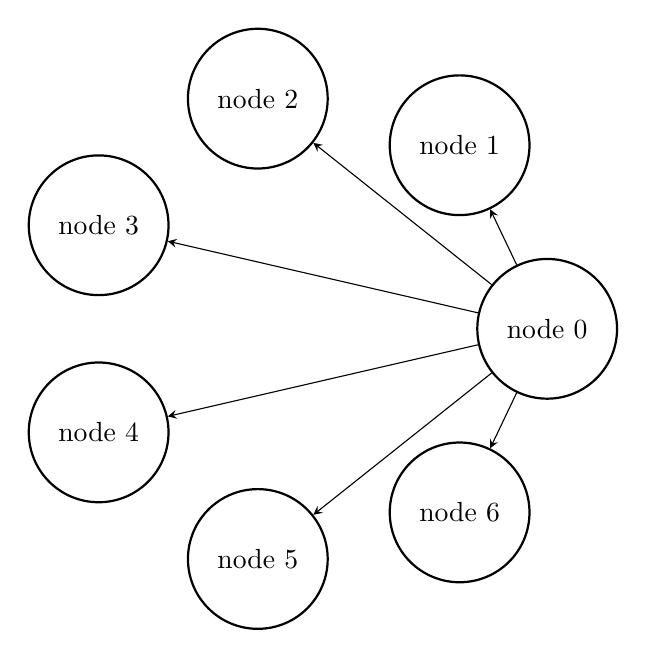
\begin{tikzpicture}[node distance=0.5cm,auto,>=stealth]
	\begin{scope}[baseline=(current bounding box.center)]
		\tikzstyle{knode}=[circle,draw=black,thick,inner sep=8pt,baseline=(current bounding box.center)]
		\node[knode] (n0) at (0:3cm) {node 0};
		\node[knode] (n1) at (51:3cm) {node 1};
		\node[knode] (n2) at (103:3cm) {node 2};
		\node[knode] (n3) at (154:3cm) {node 3};
		\node[knode] (n4) at (206:3cm) {node 4};
		\node[knode] (n5) at (257:3cm) {node 5};
		\node[knode] (n6) at (309:3cm) {node 6};
		%arrows
		\draw[->] (n0)--(n1);
		\draw[->] (n0)--(n2);
		\draw[->] (n0)--(n3);
		\draw[->] (n0)--(n4);
		\draw[->] (n0)--(n5);
		\draw[->] (n0)--(n6);
	\end{scope}
\end{tikzpicture}

	\caption{A reduced broadcast network communication pattern (single broadcast)}
	\label{fig:bcRedCommPattern}
\end{figure*}

In the following section, we compare \MessageVortex{} mimicking a BCN to a traditional BCN. We assume again that the transport layer is steganographically secured comparable to \MessageVortex.

In such a case, we may conclude that \MessageVortex{} scores over a BCN...
\begin{itemize}
	\item Equal detectability due to timing-related constraints.\\
	If \MessageVortex{} is mimicking a BCN, timing is essential. Therefore, detectability remains the same for both systems. We could argue that a \MessageVortex{} could mimic an adapted version of a BCN not working in epochs and just mimicking the communication pattern. While this would make a difference in traceability, it does not affect detectability positively or negatively.
	\item No detectability due to constant sizing of the messages.\\
	Traditional BCNs have fixed message sizes. \MessageVortex{} may mimic the communication pattern with or without such a restriction. The message size may not leak any properties when using \MessageVortex{}. Messages may travel in parts or as a whole piece.
	\item Possible resistance against a Byzantine node.
	A Byzantine node may disrupt communication in a standard BCN by flooding the network. On the other hand, \MessageVortex{} may compensate for such behavior with the possibility of redundant data. If we assume that a Byzantine node is not flooding the network completely, a BCN is likely more robust than a network of \VortexNodes{}. A BCN will score at least better if the direct path between the sender and recipient is not affected by the Byzantine node. 
	\item Possibility of redundant routes ($addRedundancy$ operation or just redundant message transfer).\\
	Messages are transferred as a block. The possibility of redundant routes is typically not foreseen in a BCN.
	\item Possibility of monitoring successful delivery.\\
	By default, a node has no means to observe successful delivery in a BCN. Using \MessageVortex{}, we may do this either by implicit or explicit diagnostic covering one or more epochs.
	\item Able to build a localized trust relationship for routing nodes over time.\\
	As we can identify successful message delivery within \MessageVortex{}, we may build a localized trust. A traditional BCN lacks this possibility. Extended networks such as ATOM may surpass this limitation.
\end{itemize}

To conclude, \MessageVortex{} may offer at least the same properties as a BCN or cBCN. Unlike ATOMt is unable to offer zero-knowledge proofs. As an alternative, \MessageVortex{} offers diagnostics. By using multi-path message transfer, \MessageVortex{} may reduce bandwidth waste and improve throughput. These capabilities of \MessageVortex{} come at the price of local node storage, complex routing operations, and RBB strategies. On the other hand, processing and scalability of \MessageVortex{} do surpass ATOM'S capability by far as the rather complex processing of ATOM is very limiting.

\chapter{Recommendations on Using the \MessageVortex{} Protocol}
The following sections list recommendations using the \MessageVortex{} protocol. It is a summary of the previous sections.

\section{Reuse of Routing Blocks\label{sec:reuseRB}}
Routing blocks should not be reused. The reuse of a routing block may leak some limited information to an adversary node, such as the approximate message size or message frequency of an unknown tupel using this network.

\section{Use of Ephemeral Identities}
Ephemeral identities should be used for a minimal number of messages. Using multiple identities with overlapping lifespans is considered a good practice. Using different ephemeral identities for the same message is acceptable and can be a good practice as long as operations do not leak the linking between those two identities.

Special care must be taken if using overlapping ephemeral identities across nodes. While ephemeral identities may be completely unlinked on a single node, linking multiple nodes may leave a trace from one identity to the next. It is advisable to recreate regularly all ephemeral identities from scratch. This guarantees an unlinking from previous ephemeral identities.

\section{Recommendations on Operations Applied on Nodes}
All operations carried out on a single node have to be crafted so that no information, whether the operation is a decoy or a real message, is leaked. Otherwise, it becomes possible to narrow down the message flow.

Encryption operations should be either strictly encrypting or strictly decrypting. At no point in the path, a previously applied encryption on an untrusted node should be removed as removal might lead to linking to the previous inverse operation.

Similarly, there are rules for adding and removing redundancy information. As these operations serve as decoy traffic generators, great care needs to be taken not to leak this information. Again, we emphasize that it is possible to add redundancy information on one node, encrypt one or multiple blocks once, or multiple blocks on a second node, and then remove the redundancy information again from the new set. This will lead to a payload data block than the original. However, this does not qualify the block as decoy traffic. The process may be reversed on the final recipient. However, such an operation is mathematically very demanding if the same operation is used for redundancy at the same time as multiple possible tuples need to be tried if one node has failed.

Whenever possible, the reappearance of a payload block in a single encoding should be avoided or limited to an absolute minimum. Such an occurrence allows the linking of two ephemeral identities.

\section{Reuse of Keys, IVs, or Routing Patterns}
An RBB should avoid the reuse of any keys, IVs, routing patterns, or PRNG seeds along its routing path of untrusted nodes. Reusing such values would allow an attacker to match ephemeral identities to a single identity. While this is minimal risk and may be ignored in some cases, an RBB should avoid it as it may leak information to collaborating nodes.

\section{Recommendations on Choosing involved Nodes}
Involved nodes should be trustworthy but not necessarily trusted. A message should always include a set of known recipients. It is regarded as good practice to use a minimal fixed anonymity set of known recipients as routers. Doing so does not leak any information unless always the same pattern of operations is applied (see \cref{sec:reuseRB}).

\section{Message Content}
Although it is possible to embed any content into a \VortexMessage, great care should be taken as the content may allow disclosing a reader's identity or location. For this reason, only self-contained messages should be used (such as plaintext messages).

Allowing a user to use more complex representations such as MIME offers many possibilities for the bugging of the content. A client displaying such messages should always handle them with great care. Taping messages by downloading external images or verifying the validity by OCSP, or even doing a reverse lookup on an IP address may leak valuable information.

\subsection{Splitting Message Content}
Message content should be split and distributed among routing nodes. Splitting should, however, not be done excessively to avoid failure due to too many failing nodes. It furthermore makes diagnostics complicated. 

\section{Routing}
The basics of routing are described in \cref{sec:routingLayer}. We collect in the following sections the recommendations regarding the routing strategies.

\subsection{Redundancy}
Redundancy is a valuable feature of the protocol. It allows unsuspicious decoy generation and to compensate message path disruption. A routing block should always be crafted so that redundancy is aligned with the complexity of the routing block and the importance of a message to avoid an adversary controlling all nodes except for the sender's and receiver's one.

Furthermore, predeployed diagnosis blocks within the message path are a good possibility to simplify the possibility of explicit routing diagnosis.

\subsection{Operation Considerations}
Operations should be kept easy, but at the same time, guarantee anonymity. The following recommendations are kept to an absolute minimum in order not to create any identifiable behavior.

A payload block should always have a single representation only once when traveling through routing nodes. A recurring pattern would allow an evil router to identify and thus match an ephemeral identity of one router to an ephemeral identity of another router, even if there are multiple routes in between. So, when applying encryption only operations between routing nodes, the encryption should be onionized. A clear onionizing routing pattern (only showing encryption steps on a single chunk) is OK. A pattern such as removing encryption and then reapply different encryption is not.

\subsection{Anonymity}
Anonymity is greatly dependent on the routing block's quality and the chosen anonymity set for a single message and a communication tuple over time. 

\hiddensubsubsection{Size of the Anonymity Set}
The requirement for an anonymity set is dependent on jurisdictional restrictions. In some of the more restrictive countries, no one can be held accountable for an action that may not be credibly assigned to him alone. In other jurisdictions, it is possible to be held liable for actions just because of an identified membership in a group. This makes it essential that message traffic and the crafting of the blending is under the sole control of the sender. He needs to create an anonymity set sufficiently large and spanning enough jurisdictions to create sufficient anonymity for his situation.
